% !TeX spellcheck = sv_SE
%http://www.cs.put.poznan.pl/ksiek/latexmath.html
%https://en.wikibooks.org/wiki/LaTeX/Advanced_Mathematics
%http://www.maths.lth.se/matematiklth/personal/magnusa/kurser/endim-ht2015/B1/kurspmB1ht15.pdf

\documentclass[a4paper]{article} 
\usepackage[T1]{fontenc} 
\usepackage[utf8]{inputenc} 
\usepackage[swedish]{babel} 
\usepackage[fleqn]{amsmath}
\usepackage{amssymb}
\usepackage{cancel}
\usepackage{graphicx}
\usepackage{enumitem}
\usepackage{systeme}
\usepackage{environ}
\usepackage[top=1in, bottom=1.25in, left=1.0in, right=1.25in]{geometry}

\setlength{\parindent}{0em}
\setlength{\parskip}{1em}

\newenvironment{task}[1]
{
	\begin{description}[align=right]
		\item [#1]~~~~
}{		%input
	\end{description}
}

\newenvironment{linsys}[1]
{
	\let\oldarraycolsep\arraycolsep
	\setlength\arraycolsep{0pt}
	\left\{\begin{array}{#1}
}{
	\end{array} \right.
	\setlength\arraycolsep{\oldarraycolsep}
}


\newcommand{\vek}[1]{\overrightarrow{#1}}

\newcommand\varpm{\mathbin{\vcenter{\hbox{%
				\oalign{\hfil$\scriptstyle+$\hfil\cr
					\noalign{\kern-.5ex}					
					$\scriptscriptstyle({-})$\cr}%
			}}}}

\newcommand{\taskref}[1]{\textbf{#1}}

\newcommand{\chapter}[2]{\section*{Kapitel #1: #2}}

\newcommand{\ans}{\textbf{Svar: }}
\newcommand{\mproof}{\text{~~~~V.S.V}}
\newcommand{\proof}{~~~~V.S.V}

\DeclareMathOperator{\lra}{\Leftrightarrow}
\DeclareMathOperator{\ra}{\Rightarrow}

\let\*\relax
\DeclareMathOperator{\*}{\cdot}

\title{Linjär algebra\\ FMA420} 
\author{Emil Wihlander\\ dat15ewi@student.lu.se} 
\date{2016--05--12}

\begin{document} 
\maketitle
\pagebreak
\chapter{1}{Linjära ekvationssystem}
\begin{task}{1.1}
	Börja nerifrån och upp och lös en variabel i taget.
	\begin{align*}
		\begin{linsys}{rrrr}
			2x+&3y-& z=&5 \\ 
			  -&3y+&5z=&1 \\
			   &   &4z=&8
		\end{linsys} \lra
		\begin{cases}
			z=2 \\
			y=\frac{1-5\*2}{-3}=3 \\
			x=\frac{5+2-3\*3}{2}=-1
		\end{cases}
	\end{align*}
	
	\ans $(x,y,z)=(-1,3,2)$
\end{task}

\begin{task}{1.2}
	Gausselimination:
	\begin{align*}
		&\begin{linsys}{rrrr}
			  x-&2y+&  z=&2 \\
			 2x-&6y+&11z=&35 \\
			-3x+&5y+&  z=&8
		\end{linsys}
		&\begin{array}{l} 
			(a) \\ 
			(b) \\
			(c)
		\end{array} \\ \lra
		&\begin{linsys}{rrrr}
			x-&2y+& z=&2 \\
			 -&2y+&9z=&31 \\
			 -& y+&4z=&14
		\end{linsys} 
		&\begin{array}{l} 
			(a')=(a) \\ 
			(b')=(b)-2(a) \\
			(c')=(c)+3(a)
		\end{array} \\ \lra
		&\begin{linsys}{rrrr}
			x-&2y+& z=&2 \\
			 -&2y+&9z=&31 \\
			  &  -&\frac{1}{2}z=&-\frac{3}{2}
		\end{linsys}
		&\begin{array}{l} 
			(a'')=(a') \\ 
			(b'')=(b') \\
			(c'')=(c')-\frac{1}{2}(b')
		\end{array} \\ \lra
		&\begin{cases}
			z=3 \\
			y=\frac{31-9\*3}{-2} =-2\\
			x=2+2\*(-2)-3=-5
		\end{cases}
	\end{align*}
		
	\ans $(x,y,z)=(-5,-2,3)$
\end{task}

\begin{task}{1.3}
	Gausselimination:
	\begin{align*}
		&\systeme{
			x-2y+ z=1,
			2x-6y+6z=2,
			-3x+5y+ z=3}  
		&\begin{array}{l} 
			(a) \\ 
			(b) \\
			(c)
		\end{array} \\ \lra
		&\systeme{
			x-2y+ z=1,
			-2y+4z=0,
			- y+4z=6}  
		&\begin{array}{l} 
			(a')=(a) \\ 
			(b')=(b)-2(a) \\
			(c')=(c)+3(a)
		\end{array} \\ \lra
		&\systeme{
			x-2y+ z=1,
			-2y+4z=0,
			2z=6}  
		&\begin{array}{l} 
			(a'')=(a') \\ 
			(b'')=(b') \\
			(c'')=(c')-\frac{1}{2}(b')
		\end{array} \\ \lra
		&\begin{cases}
			z=3 \\
			y=\frac{-4\*3}{-2} =6\\
			x=1+2\*6-3=10
		\end{cases}
	\end{align*}
		
	\ans $(x,y,z)=(10,6,3)$
\end{task}

\pagebreak

\begin{task}{1.4}
	Gausselimination:
	\begin{align*}
		&\begin{linsys}{rrrr}
			  x-&2y+& z=&1 \\
			 2x-&6y+&6z=&2 \\
			-3x+&5y-& z=&3
		\end{linsys}
		&\begin{array}{l} 
			(a) \\ 
			(b) \\
			(c)
		\end{array} \\ \lra
		&\begin{linsys}{rrrr}
			x-&2y+& z=&1 \\
			 -&2y+&4z=&0 \\
			 -& y+&2z=&6
		\end{linsys}
		&\begin{array}{l} 
			(a')=(a) \\ 
			(b')=(b)-2(a) \\
			(c')=(c)+3(a)
		\end{array} \\ \lra
		&\begin{linsys}{rrrr}
			x-&2y+& z=&1 \\
			 -&2y+&4z=&0 \\
			  &   &0z=&6
		\end{linsys}
		&\begin{array}{l} 
			(a'')=(a') \\ 
			(b'')=(b') \\
			(c'')=(c')-\frac{1}{2}(b')
		\end{array}
	\end{align*}
	Saknar lösning eftersom $0\neq6$.
	
	\ans Lösning saknas
\end{task}

\begin{task}{1.5}
	Gausselimination:
	\begin{align*}
		&\begin{linsys}{rrrr}
			 2x-&6y+&11z=&35 \\
			  x-&2y+&  z=&2 \\
			-3x+&5y+&  z=&8
		\end{linsys}
		&\begin{array}{l} 
			(a) \\ 
			(b) \\
			(c)
		\end{array} \\ \lra
		&\begin{linsys}{rrrr}
		  x-&2y+&  z=&2 \\
		 2x-&6y+&11z=&35 \\
		-3x+&5y+&  z=&8
		\end{linsys}
		&\begin{array}{l} 
			(a')=(b) \\ 
			(b')=(a) \\
			(c')=(c)
		\end{array}
	\end{align*}
	Lös som i \taskref{1.2}
	
	\ans $(x,y,z)=(-5,-2,3)$
\end{task}

\begin{task}{1.6}
	Gausselimination:
	\begin{align*}
		&\begin{linsys}{rrrr}
			  x-&2y+&3z=&1 \\
			 2x-&4y+&7z=&3 \\
			-3x+&5y-& z=&2
		\end{linsys}
		&\begin{array}{l} 
			(a) \\ 
			(b) \\
			(c)
		\end{array} \\ \lra
		&\begin{linsys}{rrrr}
			x-&2y+&3z=&1 \\
			  &   & z=&1 \\
			 -& y+&8z=&5
		\end{linsys} 
		&\begin{array}{l} 
			(a')=(a) \\ 
			(b')=(b)-2(a) \\
			(c')=(c)+3(a)
		\end{array} \\ \lra
		&\begin{linsys}{rrrr}
			x-&2y+&3z=&1 \\
			 -& y+&8z=&5 \\
			  &   & z=&1
		\end{linsys}
		&\begin{array}{l} 
			(a'')=(a') \\ 
			(b'')=(c') \\
			(c'')=(b')
		\end{array} \\ \lra
		&\begin{cases}
			z=1 \\
			y=-(5-8\*1)=3\\
			x=1+2\*3-3\*1=4
		\end{cases}
	\end{align*}
	
	\ans $(x,y,z)=(4,3,1)$
\end{task}

\begin{task}{1.7}
	Gausselimination:
	\begin{align*}
		&\begin{linsys}{rrrrr}
			  x-& y-&2z+& 2w=&-1 \\
			-3x+&4y+&7z-&12w=&2 \\
			 2x-&4y-&3z-& 2w=&-12 \\
			 5x-& y-&3z-&31w=&-20
		\end{linsys}
		&\begin{array}{l} 
			(a) \\ 
			(b) \\
			(c) \\
			(d)
		\end{array} \\ \lra
		&\begin{linsys}{rrrrr}
			x-& y-&2z+& 2w=&-1 \\
			  & y+& z-& 6w=&-1 \\
			 -&2y+& z-& 6w=&-10 \\
			  &4y+&7z-&41w=&-15
		\end{linsys}
		&\begin{array}{l} 
			(a')=(a) \\ 
			(b')=(b)+3(a) \\
			(c')=(c)-2(a) \\
			(d')=(d)-5(a)
		\end{array} \\ \lra
		&\begin{linsys}{rrrrr}
			x-&y-&2z+& 2w=&-1 \\
			  &y+& z-& 6w=&-1 \\
			  &  &3z-&18w=&-12 \\
			  &  &3z-&17w=&-11
		\end{linsys}
		&\begin{array}{l} 
			(a'')=(a') \\ 
			(b'')=(b') \\
			(c'')=(c')+2(b') \\
			(d'')=(d')-4(b')
		\end{array} \\ \lra
		&\begin{linsys}{rrrrr}
			x-&y-&2z+& 2w=&-1 \\
			  &y+& z-& 6w=&-1 \\
			  &  &3z-&18w=&-12 \\
			  &  &   &  w=&1
		\end{linsys}
		&\begin{array}{l} 
			(a''')=(a'') \\ 
			(b''')=(b'') \\
			(c''')=(c'') \\
			(d''')=(d'')-(c'')
		\end{array} \\ \lra
		&\begin{cases}
			w=1 \\
			z=\frac{-12+18\*1}{3}=2 \\
			y=-1-2+6\*1=3\\
			x=-1+3+2\*2-2\*1=4
		\end{cases}
	\end{align*}
	
	\ans $(x,y,z,w)=(4,3,2,1)$
\end{task}

\begin{task}{1.8}
	Eftersom det endast är två variabler krävs endast två ekvationer för att lösa systemet. Testa sedan mot resterande ekvationer för att se om systemet har en lösning.
	
	Gausselimination:
	\begin{align*}
		&\begin{linsys}{rrr}
			  x-&2y=&1 \\
			 3x+&4y=&13 \\
			-5x+&2y=&-13 \\
			 4x-&3y=&9
		\end{linsys}
		&\begin{array}{l} 
			(a) \\ 
			(b) \\
			(c) \\
			(d)
		\end{array} \\ \lra
		&\begin{linsys}{rrr}
			x-& 2y=&1 \\
			  &10y=&10
		\end{linsys}
		&\begin{array}{l} 
			(a')=(a) \\ 
			(b')=(b)-3(a)
		\end{array} \\ \lra
		&\begin{cases}
			y=1 \\
			x=1+2\*1=3
		\end{cases}
	\end{align*}

	Kolla $(c)$ och $(d)$:
	\[-5*3+2*1=-13\]
	\[4*3-3*1=9\]
	
	\ans $(x,y)=(3,1)$
\end{task}

\pagebreak
\begin{task}{1.9}
	Eftersom det endast är två variabler krävs endast två ekvationer för att lösa systemet. Testa sedan mot sista ekvationen för att se om systemet har en lösning.
	
	Gausselimination:
	\begin{align*}
		&\begin{linsys}{rrr}
			 x+& y=&-4 \\
			 x-&2y=&2 \\
			3x+&4y=&1
		\end{linsys}
		&\begin{array}{l} 
			(a) \\ 
			(b) \\
			(c)
		\end{array} \\ \lra
		&\begin{linsys}{rrr}
			x+& y=&-4 \\
			 -&3y=&6
		\end{linsys}
		&\begin{array}{l} 
			(a')=(a) \\ 
			(b')=(b)-(a)
		\end{array} \\ \lra
		&\begin{cases}
			y=-2 \\
			x=-2
		\end{cases}
	\end{align*}
	Kolla $(c)$:
	\[3\*(-2)+4\*(-2)=-14\neq1 \Rightarrow \text{ Saknar lösning}\]
	
	\ans Saknar lösning
\end{task}

\begin{task}{1.10}
	Eftersom det endast är tre variabler krävs endast tre ekvationer för att lösa systemet. Testa sedan mot sista ekvationen för att se om systemet har en lösning.
	
	Gausselimination:
	\begin{align*}
		&\begin{linsys}{rrrr}
			 x+&2y-& z=&1 \\
			3x-& y-&2z=&9 \\
			3x+&4y-&7z=&-5\\
			2x-&2y-& z=&7
		\end{linsys}
		&\begin{array}{l} 
			(a) \\ 
			(b) \\
			(c) \\
			(d)
		\end{array} \\ \lra
		&\begin{linsys}{rrrr}
			x+&2y-&  z=&1 \\
			 -&7y+&  z=&6 \\
			 -&2y+&10z=&-8
		\end{linsys}
		&\begin{array}{l} 
			(a')=(a) \\ 
			(b')=(b)-3(a) \\
			(c')=(c)-3(a)
		\end{array} \\ \lra
		&\begin{linsys}{rrrr}
			x+&2y-&  z=&1 \\
			 -&7y+&  z=&6 \\
			  &   &\frac{68}{7}z=&-\frac{68}{7}
		\end{linsys}
		&\begin{array}{l} 
			(a'')=(a') \\ 
			(b'')=(b') \\
			(c'')=(c')-\frac{2}{7}(b')
		\end{array} \\ \lra
		&\begin{cases}
			z=-1 \\
			y=-\frac{6+1}{7}=-1 \\
			x=1-2\*(-1)+(-1)=2
		\end{cases}
	\end{align*}
	Kolla $(d)$:
	\[2\*2-2\*(-1)-(-1)=7\]
	
	\ans $(x,y,z)=(2,-1,-1)$
\end{task}

\begin{task}{1.11}
	Gausselimination:
	\begin{align*}
		&\begin{linsys}{rrrr}
			  x-&2y+& z=&1 \\
			 2x-&6y+&6z=&4 \\
			-3x+&5y-& z=&-2
		\end{linsys}
		&\begin{array}{l} 
			(a) \\ 
			(b) \\
			(c) 
		\end{array} \\ \lra
		&\begin{linsys}{rrrr}
			x-&2y+& z=&1 \\
			 -&2y+&4z=&2 \\
			 -& y+&2z=&1
		\end{linsys}
		&\begin{array}{l} 
			(a')=(a) \\ 
			(b')=(b)-2(a) \\
			(c')=(c)+3(a)
		\end{array} \\ \lra
		&\begin{linsys}{rrrr}
			x-&2y+& z=&1 \\
			 -&2y+&4z=&2 \\
			  &   &0z=&0
		\end{linsys}
		&\begin{array}{l} 
			(a'')=(a') \\ 
			(b'')=(b') \\
			(c'')=(c')-\frac{1}{2}(b')
		\end{array}
	\end{align*}
	Alla $z$ löser $(c'')$ så låt $t$ vara ett godtyckligt tal och $z= t$. \\
	$(b'')$ ger:
	\[y=\frac{2-4t}{-2}=2t-1\]
	$(a'')$ ger:
	\[x=1+2(2t-1)-t=3t-1\]
	
	\ans $(x,y,z)=(3t-1,2t-1,t)$
\end{task}

\begin{task}{1.12}
	Gausselimination:
	\begin{align*}
		&\begin{linsys}{rrrr}
			 x-& y+&2z=&4 \\
			2x+& y-& z=&1 \\
			3x+&3y-&4z=&-2
		\end{linsys}
		&\begin{array}{l} 
			(a) \\ 
			(b) \\
			(c) 
		\end{array} \\ \lra
		&\begin{linsys}{rrrr}
			x-& y+& 2z=&4 \\
			  &3y-& 5z=&-7 \\
			  &6y-&10z=&-14
		\end{linsys}
		&\begin{array}{l} 
			(a')=(a) \\ 
			(b')=(b)-2(a) \\
			(c')=(c)-3(a)
		\end{array} \\ \lra
		&\begin{linsys}{rrrr}
			x-& y+&2z=&4 \\
			  &3y-&5z=&-7 \\
			  &   &0z=&0
		\end{linsys}
		&\begin{array}{l} 
			(a'')=(a') \\ 
			(b'')=(b') \\
			(c'')=(c')-2(b')
		\end{array}
	\end{align*}
	Alla $z$ löser $(c'')$ så låt $t$ vara ett godtyckligt tal och $z=5-3t$. \\
	$(b'')$ ger:
	\[y=\frac{-7+5(5-3t)}{3}=6-5t\]
	$(a'')$ ger:
	\[x=4+(6-5t)-2(5-3t)=t\]

	\ans $(x,y,z)=(t,6-5t,5-3t)$
\end{task}

\pagebreak
\begin{task}{1.13}
	Gausselimination:
	\begin{align*}
		&\begin{linsys}{rrrr}
			x+&2y-& z=&3 \\
			x-& y+&2z=&6
		\end{linsys}
		&\begin{array}{l} 
		(a) \\ 
		(b) 
		\end{array} \\ \lra
		&\begin{linsys}{rrrr}
			x+&2y-& z=&3 \\
			 -&3y+&3z=&3
		\end{linsys}
		&\begin{array}{l} 
		(a')=(a) \\ 
		(b')=(b)-(a) 
		\end{array} 
	\end{align*}
	Låt $t$ vara ett godtyckligt tal och $z=t$. \\
	$(b')$ ger:
	\[y=\frac{3-3t}{-3}=t-1\]
	$(a')$ ger:
	\[x=3-2(t-1)+t=5-t\]

	\ans $(x,y,z)=(5-t,t-1,t)$
\end{task}

\begin{task}{1.14}
	Gausselimination:
	\begin{align*}
		&\begin{linsys}{rrrr}
			2x+&3y+&4z=&5 \\
			4x-&3y+&2z=&1
		\end{linsys}
		&\begin{array}{l} 
			(a) \\ 
			(b) 
		\end{array} \\ \lra
		&\begin{linsys}{rrrr}
			2x+&3y+&4z=&5 \\
			  -&9y-&6z=&-9
		\end{linsys}
		&\begin{array}{l} 
			(a')=(a) \\ 
			(b')=(b)-2(a) 
		\end{array}
	\end{align*}
	Låt $t$ vara ett godtyckligt tal och $z=3t$. \\
	$(b')$ ger:
	\[y=\frac{-9+6\*3t}{-9}=1-2t\]
	$(a')$ ger:
	\[x=\frac{5-3(1-2t)-4\*3t}{2}=1-3t\]

	\ans $(x,y,z)=(1-3t,1-2t,3t)$
\end{task}

\begin{task}{1.15}
	Eftersom systemet redan är trappformat kan inte gausselimination användas för att förenkla det mer.
	\begin{align*}
		&\begin{linsys}{rrrrr}
			x+&2y+&3z+&4w=&1 \\
			  & y-&3z-& w=&5
		\end{linsys}
		&\begin{array}{l} 
			(a) \\ 
			(b) 
		\end{array}
	\end{align*}
	Låt $t$ och $s$ vara godtyckliga tal, $z=s$ och $w=t$. \\
	$(b)$ ger:
	\[y=5+3s+t\]
	$(a')$ ger:
	\[x=1-4t-3s-2(5+3s+t)=-9-9s-6t\]

	\ans $(x,y,z)=(-9-9s-6t,5+3s+t,s,t)$
\end{task}

\begin{task}{1.16}
	Gausselimination:
	\begin{align*}
		&\begin{linsys}{rrrrrr}
			 2x_1+& x_2-& x_3+&3x_4-&3x_5=&0 \\
			 3x_1+&2x_2+& x_3+&2x_4+&2x_5=&0 \\
			-4x_1+&3x_2+&2x_3+& x_4-&4x_5=&0
		\end{linsys}
		&\begin{array}{l} 
			(a) \\ 
			(b) \\
			(c)
		\end{array} \\ \lra
		&\begin{linsys}{rrrrrr}
		2x_1+&           x_2-&           x_3+&          3x_4-&           3x_5=&0 \\
		     &\frac{1}{2}x_2+&\frac{5}{2}x_3-&\frac{5}{2}x_4+&\frac{13}{2}x_5=&0 \\
		     &          5x_2+&               &          7x_4-&          10x_5=&0
		\end{linsys}
		&\begin{array}{l} 
			(a')=(a) \\
			(b')=(b)-\frac{3}{2}(a) \\
			(c')=(c)+2(a)
		\end{array} \\ \lra
		&\begin{linsys}{rrrrrr}
			2x_1+&           x_2-&           x_3+&          3x_4-&           3x_5=&0 \\
			     &\frac{1}{2}x_2+&\frac{5}{2}x_3-&\frac{5}{2}x_4+&\frac{13}{2}x_5=&0 \\
			     &              -&         25x_3+&         32x_4-&          75x_5=&0
		\end{linsys}
		&\begin{array}{l} 
			(a'')=(a') \\ 
			(b'')=(b') \\
			(c'')=(c')-10(a)
		\end{array} 
	\end{align*}
	Låt $t_1$ och $t_2$ vara godtyckliga tal, $x_4=25t_1$ och $x_5=t_2$. \\
	$(c'')$ ger:
	\[x_3=\frac{-32\*25t_1+75t_2}{-25}=32t_1-3t_2\]
	$(b'')$ ger:
	\[x_2=2(-\tfrac{5}{2}(32t_1-3t_2)+\frac{5}{2}\*25t_1-\frac{13}{2}t_2)=2t_2-35t_1\]
	$(a'')$ ger:
	\[x_1=\frac{1}{2}(-(2t_2-35t_1)+(32t_1-3t_2)-3\*25t_1+3\*t_2)=-4t_1-t_2\]

	\ans $(x_1,x_2,x_3,x_4,x_5)=(-4t_1-t_2,2t_2-35t_1,32t_1-3t_2,25t_1,t_2)$
\end{task}

\begin{task}{1.17}
	Då koefficienterna på diagonalen $a^2$, $a$ och $a^2-1$ framför $x$, $y$ och $z$ alla är skilda från noll kan ekvationssystemet lösas entydigt. $a$ måste alltså vara skilt från 0 och $\pm1$.
	
	Ekvationssystemet är redan trappformat vilket innebär att gausselimination inte behöver användas.
	\begin{align*}
		&\begin{linsys}{rrrr}
			a^2x+&2y+&      3z=&-1 \\
			     &ay+&  (a-1)z=&a+1 \\
			     &   &(a^2-1)z=&a+1
		\end{linsys}
		&\begin{array}{l} 
			(a) \\ 
			(b) \\
			(c)
		\end{array}
	\end{align*}
	$(c)$ ger: 
	\[z=\frac{a+1}{a^2-1}=\frac{1}{a-1}\]
	$(b)$ ger:
	\[y=\frac{a+1-(a-1)\frac{1}{a-1}}{a}=\frac{a+1-1}{a}=1\]
	$(a)$ ger:
	\[x=\frac{-1-2\*1-3(\frac{1}{a-1})}{a^2}=\frac{-3(\frac{a-1+1}{a-1})}{a^2}=\frac{-3}{a(a-1)}=\frac{3}{a(1-a)}\]
	\[(x,y,z)=\left(\frac{1}{a-1},1,\frac{3}{a(1-a)}\right),~~a\neq0,a\neq\pm1\]
	Om $a=1$ blir systemet:
	\begin{align*}
		&\begin{linsys}{rrrr}
			x+&2y+&3z=&-1 \\
			  & y+&  =&2 \\
			  &   &0z=&2
		\end{linsys}
	\end{align*}
	Saknar lösning eftersom $0\neq2$.
	Om $a=-1$ blir systemet:
	\begin{align*}
		&\begin{linsys}{rrrr}
			x+&2y+&3z=&-1 \\
			 -& y-&2z=&0 \\
			  &   &0z=&0
		\end{linsys}
		&\begin{array}{l} 
			(a') \\ 
			(b') \\
			(c')
		\end{array}
	\end{align*}
	Har oändligt många lösningar eftersom $0=0$. Låt $t$ vara ett godtyckligt tal och $z=t$.\\
	$(b')$ ger:
	\[y=-2t\]
	$(a')$ ger:
	\[x=-1-2\*(-2t)-3t=t-1\]
	\[(x,y,z)=(t-1,-2t,t),~~a=-1\]
	Om $a=0$ blir systemet:
	\begin{align*}
		&\begin{linsys}{rrrr}
			0x+&2y+&3z=&-1 \\
			   &  -& z=&1 \\
			   &  -& z=&1
		\end{linsys}
		&\begin{array}{l} 
			(a'') \\ 
			(b'') \\
			(c'')
		\end{array}
	\end{align*}
	Har oändligt många lösningar eftersom värdet på $x$ inte påverkar. Låt $t$ vara ett godtyckligt tal och $x=t$.\\
	$(b'')$ och $(c'')$ ger:
	\[z=-1\]
	$(a'')$ ger:
	\[y=\frac{-1-3\*(-1)}{2}=1\]
	\[(x,y,z)=(t,1,-1),~~a=0\]

	\ans Saknar lösning för $a=1$
	\[
	\begin{array}{rll}
		(x,y,z)&=\left(\frac{1}{a-1},1,\frac{3}{a(1-a)}\right),&a\neq0,a\neq\pm1 \\
		(x,y,z)&=(t-1,-2t,t),&a=-1 \\
		(x,y,z)&=(t,1,-1),&a=0
	\end{array}
	\]
\end{task}

\begin{task}{1.18}
	\begin{align*}
		&\begin{linsys}{rrrr}
			ax+& y+&2z=&4 \\
			 x+& y+& z=&1 \\
			 x+&ay+&2z=&0
		\end{linsys}
		&\begin{array}{l} 
			(a) \\ 
			(b) \\
			(c)
		\end{array} \\ \lra
		&\begin{linsys}{rrrr}
			ax+&       y+&     2z=&4 \\
			   &  (a-1)y+& (a-2)z=&a-4 \\
			   &(a^2-1)y+&2(a-1)z=&-4
		\end{linsys}
		&\begin{array}{l} 
			(a')=(a) \\ 
			(b')=a(b)-(a) \\
			(c')=a(c)-(a)
		\end{array} \\ \lra
		&\begin{linsys}{rrrr}
			ax+&     y+&       2z=&4 \\
			   &(a-1)y+&   (a-2)z=&a-4 \\
			   &       &(3a-a^2)z=&3a-a^2
		\end{linsys}
		&\begin{array}{l} 
			(a'')=(a') \\ 
			(b'')=(b') \\
			(c'')=(c')-(a+1)(b')
		\end{array} 
	\end{align*}
	$(c'')$ ger:
	\[z=\frac{3a-a^2}{3a-a^2}=1,~~a\not\in\{0,3\}\]
	$(b'')$ ger:
	\[y=\frac{a-4-(a-2)}{a-1}=\frac{2}{1-a},~~a\not\in\{0,1,3\}\]
	$(a'')$ ger:
	\[x=\frac{4-2-\frac{2}{1-a}}{a}=\frac{2}{a-1},~~a\not\in\{0,1,3\}\]
	Systemet är entydigt när $a\not\in\{0,1,3\}$.

	$a=0$ ger systemet:
	\begin{align*}
		&\begin{linsys}{rrrr}
			x+& y+& z=&1 \\
			  & y+&2z=&4 \\
			x+&   &2z=&0
		\end{linsys}
		&\begin{array}{l} 
			(a) \\ 
			(b) \\
			(c)
		\end{array} \\ \lra
		&\begin{linsys}{rrrr}
			x+& y+& z=&1 \\
			  & y+&2z=&4 \\
			 -& y+& z=&-1
		\end{linsys}
		&\begin{array}{l} 
			(a')=(a) \\ 
			(b')=(b) \\
			(c')=(c)-(a)
		\end{array} \\ \lra
		&\begin{linsys}{rrrr}
			x+& y+& z=&1 \\
			  & y+&2z=&4 \\
			  &   &3z=&3
		\end{linsys}
		&\begin{array}{l} 
			(a'')=(a') \\ 
			(b'')=(b') \\
			(c'')=(c')+(a)
		\end{array}
	\end{align*}
	$(c'')$ ger:
	\[z=1\]
	$(b'')$ ger:
	\[y=4-2\*1=2\]
	$(a'')$ ger:
	\[x=1-2-1=-2\]
	Systemet är entydigt när $a=0$.

	$a=1$ ger systemet:
	\begin{align*}
		&\begin{linsys}{rrrr}
			x+&y+&2z=&4 \\
			x+&y+& z=&1 \\
			x+&y+&2z=&0
		\end{linsys}
		&\begin{array}{l} 
			(a) \\ 
			(b) \\
			(c)
		\end{array} \\ \lra
		&\begin{linsys}{rrrr}
			x+&y+&2z=&4 \\
			  & -& z=&1 \\
			  &  &0z=&-4
		\end{linsys}
		&\begin{array}{l} 
			(a')=(a) \\ 
			(b')=(b)-(a) \\
			(c')=(c)-(a)
		\end{array}
	\end{align*}
	Systemet saknar lösning när $a=1$.

	$a=3$ ger systemet:
	\begin{align*}
		&\begin{linsys}{rrrr}
			3x+& y+&2z=&4 \\
			 x+& y+& z=&1 \\
			 x+&3y+&2z=&0
		\end{linsys}
		&\begin{array}{l} 
			(a) \\ 
			(b) \\
			(c)
		\end{array} \\ \lra
		&\begin{linsys}{rrrr}
			3x+& y+&2z=&4 \\
			   &2y+& z=&-1 \\
			   &8y+&4z=&-4
		\end{linsys}
		&\begin{array}{l} 
			(a')=(a) \\ 
			(b')=3(b)-(a) \\
			(c')=3(c)-(a)
		\end{array} \\ \lra
		&\begin{linsys}{rrrr}
			3x+& y+&2z=&4 \\
			   &2y+& z=&-1 \\
			   &   &0z=&0
		\end{linsys}
		&\begin{array}{l} 
			(a'')=(a') \\ 
			(b'')=(b') \\
			(c'')=(c')-4(b')
		\end{array} \\ \lra
	\end{align*}
	Låt $t$ vara ett godtyckligt tal och $z=-1-2t$.
	$(b'')$ ger:
	\[y=\frac{-1-(-1-2t)}{2}=t\]
	$(a'')$ ger:
	\[x=\frac{4-t-2(-1-2t)}{3}=\frac{6-3t}{3}=3-t\]
	Systemet har oändligt många lösningar när $a=3$.

	\ans $a=3$, $(x,y,z)=(3-t,t,-1-t)$
\end{task}

\begin{task}{1.19}
	Gausselimination:
	\begin{align*}
		&\begin{linsys}{rrr}
			x+&ay=&1 \\
			x-& y=&-1
		\end{linsys}
		&\begin{array}{l}
			(a) \\
			(b)
		\end{array} \\ \lra
		&\begin{linsys}{rrr}
			x+&    ay=&1 \\
			-&(a+1)y=&-2
		\end{linsys}
		&\begin{array}{l}
			(a')=(a) \\
			(b')=(b)-(a)
		\end{array}
	\end{align*}
	$(b')$ ger:
	\[y=\frac{2}{a+1},~~a\neq-1\]
	$(a')$ ger:
	\[x=1-a\frac{2}{a+1}=\frac{a+1-2a}{a+1}=\frac{1-a}{a+1},~~a\neq-1\]
	$a=-1$ ger systemet:
	\begin{align*}
		&\begin{linsys}{rrr}
			x-&y=&1 \\
			x-&y=&-1
		\end{linsys}
		&\begin{array}{l}
			(a) \\
			(b)
		\end{array} \\ \lra
			&\begin{linsys}{rrr}
			x-& y=&1 \\
			&0y=&-2
		\end{linsys}
		&\begin{array}{l}
			(a')=(a) \\
			(b')=(b)-(a)
		\end{array}
	\end{align*}
	När $a=-1$ saknar ekvationssystemet lösning eftersom $0\neq-2$.

	\ans $(x,y)=(\frac{1-a}{a+1},\frac{2}{a+1}),~~a\neq-1$, Saknar lösning när $a=-1$
\end{task}

\begin{task}{1.20}
	Kirchhoffs första lag ger att (notera att $I_1,I_2,I_5$ får negativa tecken för att pilarna är vända åt fel håll):
	\begin{align*}
		\begin{cases}
			I_3=-I_1-I_5 \\
			I_4=-I_2-I_5
		\end{cases}
	\end{align*}
	Kirchhoffs andra lag ger (sätt sedan in de givna värdena):
	\begin{align*}
		&\begin{linsys}{rl}
			U_3+U_4+R_5I_5-R_4I_4-R_3I_3=&0 \\
			U_3+R_1I_1-R_3I_3           =&0 \\
			U_4+R_2I_2-R_4I_4           =&0
		\end{linsys} \\ \lra
		&\begin{linsys}{rl}
			3+2+4I_5-I_4-I_3=&0 \\
			3+I_1-I_3       =&0 \\
			2+I_2-I_4       =&0
		\end{linsys} \\ \lra
		&\begin{linsys}{rl}
			-I_3-I_4+4I_5=&-5 \\
			I_1-I_3=&-3 \\
			I_2-I_4=&-2
		\end{linsys}
	\end{align*}
	Lägg nu ihop ekvationerna från första och andra lagen genom att substituera $I_3$ och $I_4$ mot $-I_1-I_5$ respektive $-I_2-I_5$.
	\begin{align*}
		&\begin{linsys}{rr}
			-(-I_1-I_5)-(-I_2-I_5)+4I_5=&-5 \\
			I_1-(-I_1-I_5)=&-3 \\
			I_2-(-I_2-I_5)=&-2 
		\end{linsys} \\ \lra
		&\begin{linsys}{rr}
			I_1+I_2+6I_5=&-5 \\
			2I_1+I_5=&-3 \\
			2I_2+I_5=&-2 
		\end{linsys}
		&\begin{array}{l}
			(a) \\
			(b) \\
			(c)
		\end{array} \\ \lra
		&\begin{linsys}{rr}
			10I_5=&-5 \\
			2I_1+I_5=&-3 \\
			2I_2+I_5=&-2 
		\end{linsys}
		&\begin{array}{l}
			(a')=2(a)-(b)-(c) \\
			(b')=(b) \\
			(c')=(c)
		\end{array}
	\end{align*}
	$(a')$ ger:
	\[I_5=-\frac{1}{2}\]
	$(b')$ ger:
	\[I_1=-\frac{3-\frac{1}{2}}{2}=-\frac{5}{4}\]
	$(c')$ ger:
	\[I_2=-\frac{2-\frac{1}{2}}{2}=-\frac{3}{4}\]
	Återgå sedan till ekvationerna för Kirchhoffs första lag för att bestämma $I_3$ och $I_4$.
	\[I_3=-(-\tfrac{5}{4})-(-\tfrac{1}{2})=\frac{7}{4}\]
	\[I_4=-(-\frac{3}{4})-(-\tfrac{1}{2})=\frac{5}{4}\]

	\ans $(I_1,I_2,I_3,I_4,I_5)=(-1.25A,-0.75A,1.75A,1.25A,-0.5A)$
\end{task}

\begin{task}{1.21 a)}
	Se det som att det måste finnas lika många av varje atomtyp och laddning på var sida och skapa ett ekvationssystem utifrån det.
	\begin{align*}
		&\begin{linsys}{rl}
			2x_1=&y_1 \\
			3x_1+3x_2+3x_3=&4y_1+2y_2+2y_3 \\
			x_2=&y_2 \\
			x_3=&y_3 \\
			-x_2-2x_3=&-2y_1-y_2
		\end{linsys}
		&\begin{array}{l}
			(Cr) \\
			(O) \\
			(N) \\
			(C) \\
			(e)
		\end{array} \\ \lra
		&\begin{linsys}{rl}
			2x_1=&y_1 \\
			-5x_1+x_2+x_3=&0 \\
			x_2=&y_2 \\
			x_3=&y_3 \\
			4x_1-2x_3=&0
		\end{linsys}
		&\begin{array}{l}
			(Cr')=(Cr) \\
			(O')=(O)-4(Cr)-2(N)-2(C) \\
			(N')=(N) \\
			(C')=(C) \\
			(e')=(e)+(N)+2(Cr)
		\end{array} \\ \lra
	\end{align*}
	Eftersom systemet är underbestämt kommer en variabel behövas användas för att lösa systemet. Låt därför $t$ vara ett godtyckligt tal och $x_1=t$.
	
	$(Cr')$ ger:
	\[y_1=2t\]
	$(e')$ ger:
	\[x_3=\frac{4t}{2}=2t\]
	$(C')$ ger:
	\[y_3=2t\]
	$(O')$ ger:
	\[x_2=5t-2t=3t\]
	$(N')$ ger:
	\[y_2=3t\]
	Lösningen är inte entydig.

	\ans $(x_1,x_2,x_3,y_1,y_2,y_3)=(t,3t,2t,2t,3t,2t)$
\end{task}

\begin{task}{b)}
	Se det som att det måste finnas lika många av varje atomtyp och laddning på var sida och skapa ett ekvationssystem utifrån det.
	\begin{align*}
		&\begin{linsys}{rl}
			6x_1=&12y_1 \\
			5x_1+x_3+2x_4=&10y_1+3y_2 \\
			x_1=&2y_1 \\
			2x_1+x_3+x_4=&3y_2 \\
			x_2=&y_2 \\
			-x_3=&-3y_2
		\end{linsys}
		&\begin{array}{l}
			(C) \\
			(H) \\
			(N) \\
			(O) \\
			(Zn) \\
			(e)
		\end{array} \\ \lra
		&\begin{linsys}{rl}
			x_1=&2y_1 \\
			-2x_1+x_4=&0 \\
			x_1=&2y_1 \\
			2x_1+x_4=&2y_2 \\
			x_2=&y_2 \\
			-x_3=&-y_2
		\end{linsys}
		&\begin{array}{l}
			(C')=\frac{1}{6}(C) \\
			(H')=(H)-5(N)-(O) \\
			(N')=(N) \\
			(O')=(O)+(e) \\
			(Zn')=(Zn) \\
			(e')=(e)
		\end{array} \\ \lra
	\end{align*}
	Eftersom är $(C')$ och $(N')$ är identiska är systemet underbestämt och en variabel kommer behövas användas för att lösa systemet. Låt därför $t$ vara ett godtyckligt tal och $x_1=2t$.
	
	$(C')$ och $(N')$ ger:
	\[y_1=t\]
	$(H')$ ger:
	\[x_4=2\*2t=4t\]
	$(O')$ ger:
	\[y_2=\frac{2\*2t+4t}{2}=4t\]
	$(Zn')$ ger:
	\[x_2=4t\]
	$(e')$ ger:
	\[x_3=4t\]

	\ans Allmän lösning $(x_1,x_2,x_3,x_4,y_1,y_2)=(2t,4t,4t,4t,t,4t)$
\end{task}

\begin{task}{1.22}
	\ans
\end{task}

\begin{task}{1.23}
	\ans
\end{task}

\begin{task}{1.24}
	\ans
\end{task}

\begin{task}{1.25}
	\ans
\end{task}

\begin{task}{1.26}
	\ans
\end{task}
\pagebreak
\chapter{2}{Vektorer i planet och rummet}
\begin{task}{2.1 a)}
	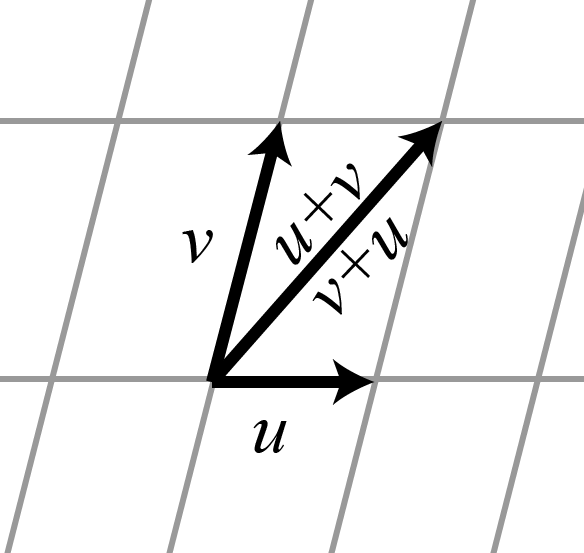
\includegraphics[scale=0.2]{images/21a.PNG}
\end{task}

\begin{task}{b)}
	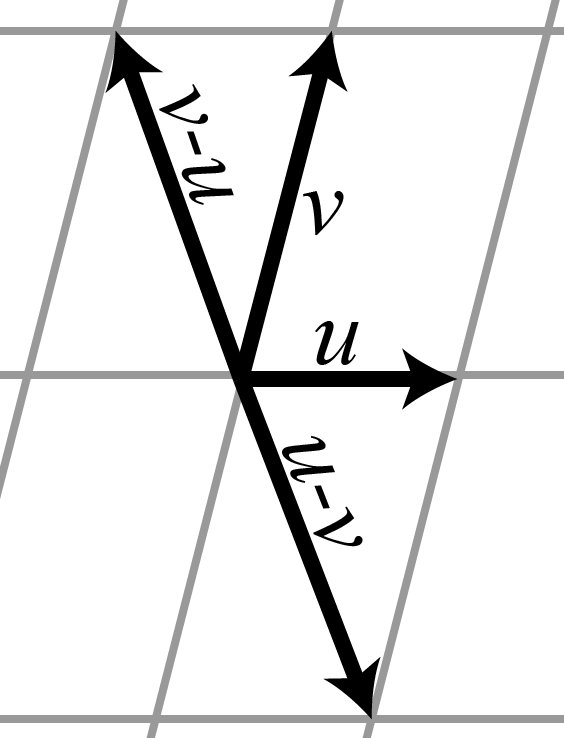
\includegraphics[scale=0.2]{images/21b.PNG}
\end{task}

\begin{task}{c)}
	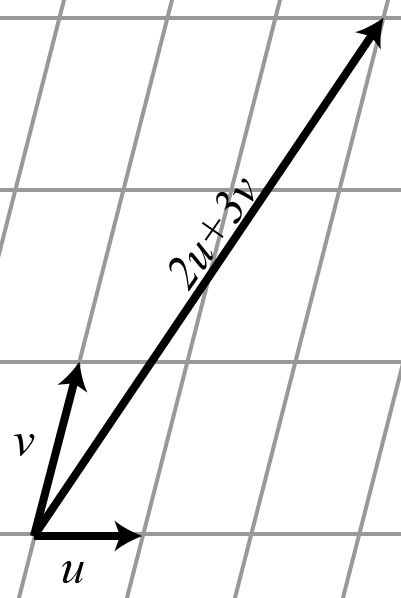
\includegraphics[scale=0.3]{images/21c.PNG}
\end{task}

\begin{task}{d)}
	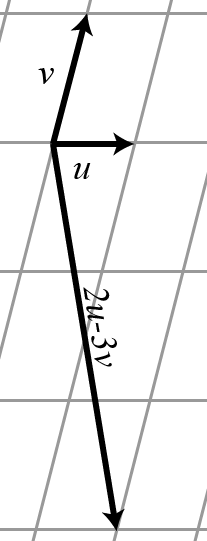
\includegraphics[scale=0.3]{images/21d.PNG}
\end{task}

\begin{task}{2.2}
	\ans Nollvektor
\end{task}

\pagebreak
\begin{task}{2.3}
	Gausselimination:
	\begin{align*}
		&\begin{linsys}{rrr}
			 \hat{u}+& \hat{v}=&u \\
			2\hat{u}+&3\hat{v}=&u
		\end{linsys}
		&\begin{array}{l}
			(a) \\
			(b)
		\end{array} \\ \lra
		&\begin{linsys}{rrr}
			\hat{u}+&\hat{v}=&u \\
			        &\hat{v}=&v-2u
		\end{linsys}
		&\begin{array}{l}
		(a')=(a) \\
		(b')=(b)-2(a)
		\end{array} \\ \lra
		&\begin{cases}
		\hat{v}=v-2u \\
		\hat{u}=u-(v-2u)=3u-v
		\end{cases}
	\end{align*}
	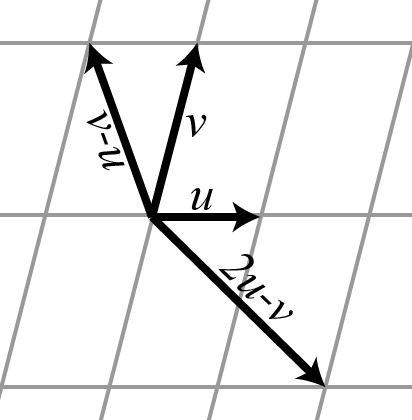
\includegraphics[scale=0.3]{images/23.PNG}
	
	\ans $\hat{v}=v-2u$, $\hat{u}=3u-v$
\end{task}

\begin{task}{2.4}
	\[\vek{OC}=\vek{OA}+\vek{AC}=\vek{OA}+\frac{1}{4}\vek{AB}\]
	\[\vek{OA}=\vek{OB}-\vek{AB} \lra
	\vek{AB}=\vek{OB}-\vek{OA}\]
	\[\vek{OC}=
	\vek{OA}+\frac{1}{4}\vek{AB}=
	\vek{OA}+\frac{1}{4}(\vek{OB}-\vek{OA})=
	\frac{3}{4}\vek{OA}+\frac{1}{4}\vek{OB} \mproof\]
\end{task}

\begin{task}{2.5}
	\[\vek{OM}=\vek{OB}-\vek{MB}=\vek{OB}-\frac{1}{2}\vek{AB}\]
	\[\vek{OB}-\vek{AB}=\vek{OA} \lra
	\vek{AB}=\vek{OB}-\vek{OA}\]
	\[\vek{OM}=
	\vek{OB}-\frac{1}{2}\vek{AB}=
	\vek{OB}-\frac{1}{2}(\vek{OB}-\vek{OA})=
	\frac{1}{2}(\vek{OB}+\vek{OA}) \mproof\]
\end{task}

\begin{task}{2.6}
	Enligt uppgiften:
	\[\vek{AM}=\frac{2}{3}\vek{AA_1}\]
	Vilket ger:
	\[\vek{OM}=
	\vek{OA}+\vek{AM}=
	\vek{OA}+\frac{2}{3}\vek{AA_1}\]
	Mittpunktsformeln:
	\[\vek{AA_1}=\frac{1}{2}(\vek{AB}+\vek{AC})\]
	Vilket ger:
	\[\vek{OM}=
	\vek{OA}+\frac{2}{3}\*\frac{1}{2}(\vek{AB}+\vek{AC})=
	\vek{OA}+\frac{1}{3}(\vek{AB}+\vek{AC})\]
	Enligt figuren:
	\[\vek{AB}=\vek{OB}-\vek{OA},~~
	\vek{AC}=\vek{OC}-\vek{OA}\]
	Vilket ger:
	\[\vek{OM}=
	\vek{OA}+\frac{1}{3}(\vek{OB}-\vek{OA}+\vek{OC}-\vek{OA})=
	\frac{1}{3}(\vek{OA}+\vek{OB}+\vek{OC}) \mproof\]
\end{task}

\begin{task}{2.7}
	Enligt uppgiften:
	\[\vek{AM}=\frac{3}{4}\vek{AA_1}\]
	Vilket ger:
	\[\vek{OM}=
	\vek{OA}+\vek{AM}=
	\vek{OA}+\frac{3}{4}\vek{AA_1}\]
	Tyngdpunktsformeln:
	\[\vek{AA_1}=\frac{1}{3}(\vek{AB}+\vek{AC}+\vek{AD})\]
	Vilket ger:
	\[\vek{OM}=
	\vek{OA}+\frac{3}{4}\*\frac{1}{3}(\vek{AB}+\vek{AC}+\vek{AD})=
	\vek{OA}+\frac{1}{4}(\vek{AB}+\vek{AC}+\vek{AD})\]
	Enligt figuren:
	\[\vek{AB}=\vek{OB}-\vek{OA},~~
	\vek{AC}=\vek{OC}-\vek{OA},~~
	\vek{AD}=\vek{OD}-\vek{OA}\]
	Vilket ger:
	\[\vek{OM}=
	\vek{OA}+\frac{1}{4}(\vek{OB}-\vek{OA}+\vek{OC}-\vek{OA}+\vek{OD}-\vek{OA})=
	\frac{1}{4}(\vek{OA}+\vek{OB}+\vek{OC}+\vek{OD}) \text{~~~~V.S.V}\]
\end{task}

\begin{task}{2.8}
	Låt $O$ ligga i punkten $M$. tyngdpunktsformeln ger:
	\[\vek{OM}=\frac{1}{3}(\vek{OA}+\vek{OB}+\vek{OC})\]
	Eftersom $O=M$:
	\[\begin{cases}
	\vek{OM}=0 \\
	\vek{OA}=\vek{MA} \\
	\vek{OB}=\vek{MB} \\
	\vek{OC}=\vek{MC}
	\end{cases}\]
	Vilket ger:
	\[\frac{1}{3}(\vek{MA}+\vek{MB}+\vek{MC})=0 \lra
	\vek{MA}+\vek{MB}+\vek{MC}=3\*0=0 \text{~~~~V.S.V}\]
\end{task}

\begin{task}{2.9}
	Låt $O$ vara en godtycklig punkt i rummet. Vilket ger:
	\[\begin{cases}
	\vek{A_1A_2}=\vek{OA_2}-\vek{OA_1} \\
	\vek{B_1B_2}=\vek{OB_2}-\vek{OB_1} \\
	\vek{C_1C_2}=\vek{OC_2}-\vek{OC_1}
	\end{cases}\]
	Tyngdpunktsformeln baklänges samt hur differens för vektorer funkar ger:
	\begin{align*}
	&\vek{A_1A_2}+\vek{B_1B_2}+\vek{C_1C_2}=
	\vek{OA_2}-\vek{OA_1}+\vek{OB_2}-\vek{OB_1}+\vek{OC_2}-\vek{OC_1}= \\ =
	&3\*\frac{1}{3}(\vek{OA_2}+\vek{OB_2}+\vek{OC_2})-3\*\frac{1}{3}(\vek{OA_1}+\vek{OB_1}+\vek{OC_1})= \\ =
	&3(\vek{OM_2}-\vek{OM_1})=
	3\vek{M_1M_2} \text{~~~~V.S.V}
	\end{align*}
\end{task}

\begin{task}{2.10}
	Mittpunktsformeln ger:
	\[\begin{cases}
	\vek{OA_m}=\frac{1}{2}(\vek{OA}+\vek{OB}) \\
	\vek{OB_m}=\frac{1}{2}(\vek{OB}+\vek{OC}) \\
	\vek{OC_m}=\frac{1}{2}(\vek{OC}+\vek{OA})
	\end{cases}\]
	Vilket ger:
	\begin{align*}
	&VL=\vek{OA_m}+\vek{OB_m}+\vek{OC_m}=
	\frac{1}{2}(\vek{OA}+\vek{OB})+\frac{1}{2}(\vek{OB}+\vek{OC})+\frac{1}{2}(\vek{OC}+\vek{OA})= \\ =
	&\frac{1}{2}(2\vek{OA}+2\vek{OB}+2\vek{OC})=
	\vek{OA}+\vek{OB}+\vek{OC}=HL \text{~~~~V.S.V}
	\end{align*}
\end{task}

\begin{task}{2.11}
	Låt $ABCD$ vara en godtycklig tetraeder i rummet och $O$ vara en godtycklig punkt i rummet. 
	Om alla sammanbindningar skär tyngdpunkt vet vi även att alla skär varandra i tyngdpunkten.
	Antag att tyngdpunkten ligger i punkten $M$ och $\vek{OM}=\frac{1}{4}(\vek{OA}+\vek{OB}+\vek{OC}+\vek{OD})$.

	Mittpunktsformeln ger:
	\[\begin{array}{lcr}
	p_1=\frac{1}{2}(\vek{OA}+\vek{OB}) & \text{~~~~motsatta punkt:~~~~} & q_1=\frac{1}{2}(\vek{OC}+\vek{OD}) \\
	p_2=\frac{1}{2}(\vek{OB}+\vek{OC}) & \text{~~~~motsatta punkt:~~~~} & q_2=\frac{1}{2}(\vek{OA}+\vek{OD}) \\
	p_3=\frac{1}{2}(\vek{OC}+\vek{OA}) & \text{~~~~motsatta punkt:~~~~} & q_3=\frac{1}{2}(\vek{OB}+\vek{OD})
	\end{array}\]
	En slumpmässig punkt på varje sammanbindning kan beskrivas som där $x,y,z$ ligger mellan 0 och 1:
	\[\begin{array}{l}
	s_1=p_1+x(q_1-p_1)=\frac{1}{2}(\vek{OA}+\vek{OB})+x\frac{1}{2}((\vek{OA}+\vek{OB})-(\vek{OC}+\vek{OD})) \\
	s_2=p_2+y(q_2-p_2)=\frac{1}{2}(\vek{OB}+\vek{OC})+y\frac{1}{2}((\vek{OB}+\vek{OC})-(\vek{OA}+\vek{OD})) \\
	s_2=p_3+z(q_3-p_3)=\frac{1}{2}(\vek{OC}+\vek{OA})+z\frac{1}{2}((\vek{OC}+\vek{OA})-(\vek{OB}+\vek{OD}))
	\end{array}\]
	Om vi sätter $x=y=z=\frac{1}{2}$ så kommer $s_1=s_2=s_3=\frac{1}{4}(\vek{OA}+\vek{OB}+\vek{OC}+\vek{OD})$ vilket är samma punkt som vi antog att tyngdpunkten $M$ skulle ligga i. Eftersom alla tre skär $M$ skär även alla tre varandra i $M$. ~~V.S.V
\end{task}

\begin{task}{2.12}
	Låt $O$ vara en godtycklig punkt i rummet. 
	Om två stycken sträckor beskriver samma vektor måste de vara parallella enligt definitionen från vektorer. 
	Så om $\vek{A_1B_1}=\vek{D_1C_1}$ och $\vek{B_1C_1}=\vek{A_1D_1}$ är $A_1B_1C_1D_1$ en parallellogram.

	mittpunktsformeln:
	\[\begin{array}{l}
	\vek{OA_1}=\frac{1}{2}(\vek{OA}+\vek{OB}) \\
	\vek{OB_1}=\frac{1}{2}(\vek{OB}+\vek{OC}) \\
	\vek{OC_1}=\frac{1}{2}(\vek{OC}+\vek{OD}) \\
	\vek{OD_1}=\frac{1}{2}(\vek{OD}+\vek{OA})
	\end{array}\]
	\[\begin{array}{l}
	\vek{A_1B_1}=\vek{OB_1}-\vek{OA_1}=\frac{1}{2}(\vek{OB}+\vek{OC}-(\vek{OA}+\vek{OB}))=\frac{1}{2}(\vek{OC}-\vek{OA}) \\
	\vek{D_1C_1}=\vek{OC_1}-\vek{OD_1}=\frac{1}{2}(\vek{OC}+\vek{OD}-(\vek{OD}+\vek{OA}))=\frac{1}{2}(\vek{OC}-\vek{OA}) \\
	\vek{B_1C_1}=\vek{OC_1}-\vek{OB_1}=\frac{1}{2}(\vek{OC}+\vek{OD}-(\vek{OB}+\vek{OC}))=\frac{1}{2}(\vek{OD}-\vek{OB}) \\
	\vek{A_1D_1}=\vek{OD_1}-\vek{OA_1}=\frac{1}{2}(\vek{OD}+\vek{OA}-(\vek{OA}+\vek{OB}))=\frac{1}{2}(\vek{OD}-\vek{OB})
	\end{array}\]
	$\vek{A_1B_1}=\vek{D_1C_1}$ och $\vek{B_1C_1}=\vek{A_1D_1}$ är alltså sant vilket innebär att $A_1B_1C_1D_1$ är en parallellogram. ~~V.S.V
\end{task}

\pagebreak
\begin{task}{2.13 a)}
	\[u_1=3e_1+2e_2\]
	
	\ans $(3,2)$
\end{task}

\begin{task}{b)}
	\[u_2=2e_1+3e_2\]
	
	\ans $(2,3)$
\end{task}

\begin{task}{c)}
	\[u_3=-2e_1+2e_2\]
	
	\ans $(-2,2)$
\end{task}

\begin{task}{d)}
	\[u_4=-3e_1-2e_2\]
	
	\ans $(-3,-2)$
\end{task}

\begin{task}{e)}
	\[u_5=2e_1-3e_2\]
	
	\ans $(2,-3)$
\end{task}

\begin{task}{f)}
	\[e_1=1e_1+0e_2\]
	
	\ans $(1,0)$
\end{task}

\begin{task}{g)}
	\[e_2=0e_1+1e_2\]
	
	\ans $(0,1)$
\end{task}

\begin{task}{2.14 a)}
	$\hat{v}=v-2u$, $\hat{u}=3u-v$
	\begin{align*}
		&u=a\hat{u}+b\hat{v}=
		a(3u-v)+b(v-2u)=
		(3a-2b)u+(b-a)v \lra \\ \lra
		&\begin{cases}
			3a-2b=1 \\
			b-a=0
		\end{cases} \lra
		\begin{cases}
			a=1 \\ 
			b=1
		\end{cases} \lra
		u=1\hat{u}+1\hat{v}
	\end{align*}
	
	\begin{align*}
		&u=a\hat{u}+b\hat{v}=
		a(3u-v)+b(v-2u)=
		(3a-2b)u+(b-a)v \lra \\ \lra
		&\begin{cases}
			3a-2b=0 \\
			b-a=1
		\end{cases} \lra
		\begin{cases}
			a=2 \\ 
			b=3
		\end{cases} \lra
		u=2\hat{u}+3\hat{v}
	\end{align*}
	
	\ans $u:~(1,1)$ och $v:~(2,3)$
\end{task}

\begin{task}{b)}
	\[\hat{u}=3u-v=3u-1v\]
	\[\hat{v}=v-2u=-2u+1v\]
	
	\ans $\hat{u}:~(3,-1)$ och $\hat{v}:~(-2,1)$
\end{task}

\begin{task}{2.15}
	\[\vek{OC}=\frac{3}{4}\vek{OA}+\frac{1}{4}\vek{OB}\]
	
	\ans $\vek{OC}:~(3/4,1/4)$
\end{task}

\begin{task}{2.16}
	För $\vek{TC}$ använd tyndpunktsformeln och låt $T$ vara den godtyckliga punkten i rummet.
	\[\vek{TT}=\frac{1}{3}(\vek{TA}+\vek{TB}+\vek{TC}) \lra
	0=\frac{1}{3}\vek{TA}+\frac{1}{3}\vek{TB}+\frac{1}{3}\vek{TC} \lra
	\vek{TC}=-\vek{TA}-\vek{TB}\]
	För $\vek{TM}$ använd mittpunktsformeln där $T$ är den godtyckliga punkten i rummet.
	\[\vek{TM}=\frac{1}{2}(\vek{TA}+\vek{TB})=\frac{1}{2}\vek{TA}+\frac{1}{2}\vek{TB}\]
	
	\ans $\vek{TC}:~(-1,-1)$ och $\vek{TM}:~(1/2,1/2)$
\end{task}

\begin{task}{2.17 a)}
	Vi ansätter lösningen:
	\[(4,1,-5)=x(2,1,-1)+y(1,1,1)\]
	Identifierar variablerna (gausselimination):
	\[\begin{cases}
		2x+y=4 \\
		x+y=1 \\
		-x+y=-5
	\end{cases} \lra
	\begin{cases}
		2x+y=4 \\
		y=-2 \\
		3y=-6
	\end{cases} \lra
	\begin{cases}
		x=3 \\
		y=-2
	\end{cases}\]
	
	\ans $(4,1,-5)$ är en linjärkombination av $u_1$ och$u_2$
\end{task}

\begin{task}{b)}
	Vi ansätter lösningen:
	\[(4,3,2)=x(2,1,-1)+y(1,1,1)\]
	Identifierar variablerna (gausselimination):
	\[\begin{cases}
		2x+y=4 \\
		x+y=3 \\
		-x+y=2
	\end{cases} \lra
	\begin{cases}
		2x+y=4 \\
		y=2 \\
		3y=0
	\end{cases} \lra
	y=2\neq0 \ra \text{ Saknar lösning.}\]
	
	\ans $(4,3,2)$ är inte en linjärkombination av $u_1$ och$u_2$
\end{task}

\begin{task}{c)}
	Vi ansätter lösningen:
	\[(-9,-7,-3)=x(2,1,-1)+y(1,1,1)\]
	Identifierar variablerna (gausselimination):
	\[\begin{cases}
		2x+y=-9 \\
		x+y=-7 \\
		-x+y=-3
	\end{cases} \lra
	\begin{cases}
		2x+y=-9 \\
		y=-5 \\
		3y=-15
	\end{cases} \lra
	\begin{cases}
		x=-7 \\
		y=-5
	\end{cases}\]
	
	\ans $(-9,-7,-3)$ är en linjärkombination av $u_1$ och$u_2$
\end{task}

\begin{task}{2.18 a)}
	För att två vektorer ska vara parallella ska det finnas ett $k$ så att:
	\[u=kv\]
	Ansätt därför en lösning och identifiera $k$ och $a$:
	\[(a,1+a)=k(2,-3) \lra
	\begin{cases}
		a=2k \\
		1+a=-3k
	\end{cases} \lra
	\begin{cases}
		a=-\frac{2}{5} \\
		k=-\frac{1}{5}
	\end{cases}\]
	
	\ans $a=-\frac{2}{5}$
\end{task}

\begin{task}{b)}
	För att två vektorer ska vara parallella ska det finnas ett $k$ så att:
	\[u=kv\]
	Ansätt därför en lösning och identifiera $k$ och $a$:
	\[(a,-3)=k(2,1-a) \lra
	\begin{cases}
		a=2k \\
		-3=k(1-a)
	\end{cases}\]
	Substitutionsmetoden:
	\[-3=k(1-2k) \lra
	2k^2-k-3=0 \lra
	k^2-\frac{k}{2}-\frac{3}{2}=0\]
	\[k=\frac{1}{4}\pm\sqrt{\frac{1}{16}+\frac{24}{16}}=\frac{1}{4}\pm\frac{5}{4}\]
	\[\begin{cases}
		k_1=\frac{3}{2} \lra a_1=3 \\
		k_2=-1 \lra a_2=-2
	\end{cases}\]
	
	\ans $a=3$ eller $a=-2$
\end{task}

\begin{task}{c)}
	För att två vektorer ska vara parallella ska det finnas ett $k$ så att:
	\[u=kv\]
	Ansätt därför en lösning och identifiera $k$ och $a$:
	\[(a,3)=k(2,1-a) \lra
	\begin{cases}
		a=2k \\
		3=k(1-a)
	\end{cases}\]
	Substitutionsmetoden:
	\[3=k(1-2k) \lra
	2k^2-k+3=0 \lra
	k^2-\frac{k}{2}+\frac{3}{2}=0\]
	\[k=\frac{1}{4}\pm\sqrt{\frac{1}{16}-\frac{24}{16}}=\frac{1}{4}\pm\sqrt{-\frac{23}{16}} \ra \text{ Saknar reell lösning}\]

	\ans Saknar lösning
\end{task}

\begin{task}{d)}
	För att två vektorer ska vara parallella ska det finnas ett $k$ så att:
	\[u=kv\]
	Ansätt därför en lösning och identifiera $k$ och $a$:
	\[(a,1+a,3)=k(4,2,-6) \lra
	\begin{cases}
		a=4k \\
		1+a=2k \\
		3=-6k
	\end{cases} \lra
	\begin{cases}
		a=4k \\
		1=-2k \\
		3=-6k
	\end{cases} \lra
	\begin{cases}
		a=-2 \\
		k=-\frac{1}{2}
	\end{cases}\]
	
	\ans $a=-2$
\end{task}

\begin{task}{2.19 a)}
	För att vektorerna ska vara linjärt beroende ska de gå att beskriva med hjälp av varandra vilket innebär att det ska finnas ett $k$ så att:
	\[(2,4)=k(-4,-2)\]
	Identifiera variabeln:
	\[\begin{cases}
		2=-4k \\
		4=-2k
	\end{cases} \lra
	k=-\frac{1}{2}\neq-2 \ra \text{ saknar lösning}\]
	
	\ans Vektorerna är inte linjärt beroende
\end{task}

\begin{task}{b)}
	För att vektorerna ska vara linjärt beroende ska de gå att beskriva med hjälp av varandra vilket innebär att det ska finnas ett $k$ så att:
	\[(6,-3)=k(-4,2)\]
	Identifiera variabeln:
	\[\begin{cases}
		6=-4k \\
		-3=2k
	\end{cases} \lra
	k=-\frac{3}{2}\]
	
	\ans Vektorerna är linjärt beroende
\end{task}

\begin{task}{c)}
	För att vektorerna ska vara linjärt beroende ska de vara parallella och enligt definition är nollvektorn $(0,0)$ parallell med alla vektorer och därför är vektorerna linjärt beroende.
	
	\ans Vektorerna är linjärt beroende
\end{task}

\begin{task}{d)}
	För att vektorerna ska vara linjärt beroende ska de gå att beskriva med hjälp av varandra vilket innebär att det ska finnas ett $k_1$ och ett $k_2$ så att:
	\[(1,0)=k_1(0,1)+k_2(7,5)\]
	Identifiera variablerna:
	\[\begin{cases}
		1=7k_2 \\
		0=k_1+5k_2
	\end{cases} \lra
	\begin{cases}
		k_1=-\frac{5}{7} \\
		k_2=\frac{1}{7}
	\end{cases} \ra \text{ linjärt beroende}\]
	
	\ans Vektorerna är linjärt beroende
\end{task}

\begin{task}{e)}
	För att vektorerna ska vara linjärt beroende ska de gå att beskriva med hjälp av varandra vilket innebär att det ska finnas ett $k_1$ och ett $k_2$ så att:
	\[(5,9)=k_1(3,-2)+k_2(2,1)\]
	Identifiera variablerna:
	\[\begin{cases}
		5=3k_1+2k_2 \\
		9=-2k_1+k_2
	\end{cases} \lra
	\begin{cases}
		k_1=-\frac{13}{7} \\
		k_2=\frac{37}{7}
	\end{cases} \ra \text{ linjärt beroende}\]
	
	\ans Vektorerna är linjärt beroende
\end{task}

\begin{task}{2.20 a)}
	För att vektorerna ska vara linjärt beroende ska de gå att beskriva med hjälp av varandra vilket innebär att det ska finnas ett $k_1$ och ett $k_2$ så att:
	\[(1,1,1)=k_1(3,1,2)+k_2(0,2,1)\]
	Identifiera variablerna:
	\[\begin{cases}
		1=3k_1+0k_2 \\
		1=k_1+2k_2 \\
		1=2k_1+k_2
	\end{cases} \lra
	\begin{cases}
		k_1=\frac{1}{3} \\
		k_2=\frac{1}{3}
	\end{cases} \ra \text{ linjärt beroende}\]
	
	\ans Vektorerna är linjärt beroende
\end{task}

\begin{task}{b)}
	För att vektorerna ska vara linjärt beroende ska de gå att beskriva med hjälp av varandra vilket innebär att det ska finnas ett $k_1$ och ett $k_2$ så att:
	\[(0,1,1)=k_1(1,0,1)+k_2(1,1,0)\]
	Identifiera variablerna:
	\[\begin{cases}
		0=k_1+k_2 \\
		1=0k_1+k_2 \\
		1=k_1+0k_2
	\end{cases} \lra
	\begin{cases}
		k_1=1 \\
		k_2=1\neq-1
	\end{cases} \ra \text{ linjärt oberoende}\]
	
	\ans Vektorerna är inte linjärt beroende
\end{task}

\begin{task}{c)}
	För att vektorerna ska vara linjärt beroende ska de gå att beskriva med hjälp av varandra vilket innebär att det ska finnas ett $k$ så att:
	\[(1,1,1)=k(3,1,2)\]
	Identifiera variabeln:
	\[\begin{cases}
		1=3k \\
		1=k \\
		1=2k
	\end{cases} \lra
	k=\frac{1}{3}\neq1\neq\frac{1}{2} \ra \text{ linjärt oberoende}\]
	
	\ans Vektorerna är inte linjärt beroende
\end{task}

\begin{task}{d)}
	För att vektorerna ska vara linjärt beroende ska de gå att beskriva med hjälp av varandra vilket innebär att det ska finnas ett $k$ så att:
	\[(1,0,2)=k(-2,0,-4)\]
	Identifiera variabeln:
	\[\begin{cases}
		1=-2k \\
		0=0k \\
		2=-4k
	\end{cases} \lra
	k=-\frac{1}{2} \ra \text{ linjärt beroende}\]
	
	\ans Vektorerna är linjärt beroende
\end{task}

\begin{task}{e)}
	Eftersom $(1,0,2)$ och $(-2,0,-4)$ är linjärt beroende (se \taskref{d)}) är även $(2,0,3)$, $(1,0,2)$ och $(-2,0,-4)$ det.
	
	\ans Vektorerna är linjärt beroende
\end{task}

\begin{task}{f)}
	För att vektorerna ska vara linjärt beroende ska de gå att beskriva med hjälp av varandra vilket innebär att det ska finnas ett $k_1$ och ett $k_2$ så att:
	\[(1,0,2)=k_1(3,0,4)+k_2(5,0,6)\]
	Identifiera variablerna (gausselimination):
	\[\begin{cases}
		1=3k_1+5k_2 \\
		0=0k_1+0k_2 \\
		2=4k_1+6k_2
	\end{cases} \lra
	\begin{cases}
		k_1=2 \\
		k_2=-1
	\end{cases}\ra \text{ linjärt beroende}\]
	
	\ans Vektorerna är linjärt beroende
\end{task}

\begin{task}{g)}
	För att vektorerna ska vara linjärt beroende ska de gå att beskriva med hjälp av varandra vilket innebär att det ska finnas ett $k_1$, ett $k_2$ och ett $k_3$ så att:
	\[(1,1,0)=k_1(1,0,1)+k_2(0,1,1)+k_3(3,3,3)\]
	Identifiera variablerna (gausselimination):
	\[\begin{cases}
		1=k_1+0k_2+3k_3 \\
		1=0k_1+k_2+3k_3 \\
		0=k_1+k_2+3k_3
	\end{cases} \lra
	\begin{cases}
		k_1=-1 \\
		k_2=-1 \\
		k_3=\frac{2}{3}
	\end{cases}\ra \text{ linjärt beroende}\]
	
	\ans Vektorerna är linjärt beroende
\end{task}

\begin{task}{2.21}
	För att vektorerna ska vara linjärt beroende ska de gå att beskriva med hjälp av varandra (de ska vara parallella) vilket innebär att det ska finnas ett $k$ och $a$ så att:
	\[(a,-2)=k(1,a-1)\]
	Identifiera variabeln:
	\[\begin{cases}
		a=k \\
		-2=k(a-1)
	\end{cases}\]
	Substitutionsmetoden:
	\[-2=k(k-1) \lra
	k^2-k+2=0\]
	\[k=\frac{1}{2}\pm\sqrt{\frac{1}{4}-\frac{8}{4}}=\frac{1}{2}\pm\sqrt{-\frac{7}{4}} \ra \text{ saknar reell lösning}\]
	
	\ans Nej, det finns inget $a$ så att vektorerna är linjärt beroende
\end{task}

\begin{task}{2.22 a)}
	\[u=5e_1+3e_2\]
	
	\ans $(5,3)$
\end{task}

\begin{task}{b)}
	Ja, eftersom de inte är parallella.
	
	\ans Ja
\end{task}

\begin{task}{c)}
	\[2\hat{e}_1+\hat{e}_2=u\]

	\ans $(2,1)$
\end{task}

\begin{task}{d)}
	\[\hat{e}_1=e_1+2e_2 \ra (1,2)\]
	\[\hat{e}_2=3e_1-e_2 \ra (3,-1)\]
	
	\ans $\hat{e}_1:~(1,2)$ och $\hat{e}_2:~(3,-1)$
\end{task}

\begin{task}{e)}
	\begin{align*}
		&x_1e_1+x_2e_2=v=
		\hat{x}_1\hat{e}_1+\hat{x}_2\hat{e}_2=
		\hat{x}_1(e_1+2e_2)+\hat{x}_2(3e_1-e_2)= \\ =
		&(\hat{x}_1+3\hat{x}_2)e_1+(2\hat{x}_1-\hat{x}_2)e_2 \ra (x_1,x_2)=(\hat{x}_1+3\hat{x}_2,2\hat{x}_1-\hat{x}_2)
	\end{align*}
\end{task}

\begin{task}{2.23}
	$\hat{e}_1$ och $\hat{e}_2$ kan användas som bas om de inte är parallella så genom att anta att de är parallella kan vi bestämma om de kan användas som bas eller inte. De är parallella om det finns ett $k$ så att:
	\[\hat{e}_1=k\hat{e}_2\] 
	\[\hat{e}_1=k\hat{e}_2 \lra
	-e_1+2e_2=k(3e_1+4e_2) \lra
	\begin{cases}
		-1=3k \\
		2=4k
	\end{cases} \lra
	k=-\frac{1}{3}\neq\frac{1}{2}\]
	Linjerna är inte parallella och därför kan de vara en bas i planet.
	\begin{align*}
		&\begin{cases}
			\hat{e}_1=-e_1+2e_2 \\
			\hat{e}_2=3e_1+4e_2
		\end{cases} \lra
		\begin{cases}
			e_1=-\hat{e}_1+2e_2 \\
			e_2=\frac{1}{4}\hat{e}_2-\frac{3}{4}e_1
		\end{cases}\lra \\ \lra
		&\begin{cases}
			e_1=-\hat{e}_1+2(\frac{1}{4}\hat{e}_2-\frac{3}{4}e_1) \\
			e_2=\frac{1}{4}\hat{e}_2-\frac{3}{4}(-\hat{e}_1+2e_2)
		\end{cases}\lra
		\begin{cases}
			e_1=-\frac{2}{5}\hat{e}_1+\frac{1}{5}\hat{e}_2 \\
			e_2=\frac{3}{10}\hat{e}_1+\frac{1}{10}\hat{e}_2
		\end{cases}
	\end{align*}
	Sätt sedan in i uttrycket för vektorn.
	\begin{align*}
		&u=4e_1-5e_2=
		4(-\frac{2}{5}\hat{e}_1+\frac{1}{5}\hat{e}_2)-5(\frac{3}{10}\hat{e}_1+\frac{1}{10}\hat{e}_2)= \\ =
		&-\frac{8}{5}\hat{e}_1-\frac{15}{10}\hat{e}_1+\frac{4}{5}\hat{e}_2-\frac{5}{10}\hat{e}_2=
		-\frac{31}{10}\hat{e}_1+\frac{3}{10}\hat{e}_2
	\end{align*}
	
	\ans $(-3.1,0.3)$
\end{task}

\pagebreak
\begin{task}{2.24 a)}
	För att visa att $e^{'}_1$, $e^{'}_2$ och $e^{'}_3$ är en bas i rummet behöver vi först visa att  $e^{'}_1$ och $e^{'}_2$ är linjärt oberoende i planet och sedan visa att $e^{'}_3$ är linjärt oberoende i rummet.
	
	Om det inte finns $k$ så att:
	\[e^{'}_1=ke^{'}_2\]
	är $e^{'}_1$ och $e^{'}_2$ linjärt oberoende i planet.
	\begin{align*}
		&e^{'}_1=ke^{'}_2 \lra
		e^1+0e^2+0e^3=k(2e^1+e^2+0e^3) \lra \\ \lra
		&\begin{cases}
			1=2k \\
			0=k \\
			0=0
		\end{cases} \lra
		k=\frac{1}{2}\neq0 \lra
		\text{ linjärt oberoende}
	\end{align*}
	Om det inte finns $k_1$ och $k_2$ så att:
	\[e^{'}_3=k_1e^{'}_1+k_2e^{'}_2\]
	är $e^{'}_1$, $e^{'}_2$ och $e^{'}_3$ linjärt oberoende i rummet.
	\begin{align*}
		&e^{'}_3=k_1e^{'}_1+k_2e^{'}_2 \lra \\ \lra
		&3e^1+2e^2+e^3=k_1(e^1+0e^2+0e^3)+k_2(2e^1+e^2+0e^3) \lra \\ \lra
		&\begin{cases}
			3=k_1+2k_2 \\
			2=k_2 \\
			1\neq0
		\end{cases} \lra
		1\neq0 \lra
		\text{ linjärt oberoende}
	\end{align*}
	\ans $e^{'}_1$, $e^{'}_2$ och $e^{'}_3$ är en bas i rummet.
\end{task}

\begin{task}{b)}
	\[x^{'}_1e^{'}_1+x^{'}_2e^{'}_2+x^{'}_3e^{'}_3=x_1e_1+x_2e_2+x_3e_3\]
	\begin{align*}
		VL=&x^{'}_1(e_1)+x^{'}_2(2e_1+e_2)+x^{'}_3(3e_1+2e_2+e_3)= \\ =
		&(x^{'}_1+2x^{'}_2+3x^{'}_3)e_1+(x^{'}_2+2x^{'}_3)e_2+x^{'}_3e_3
	\end{align*}
	identifiera variablerna:
	\[\begin{cases}
		x_1=x^{'}_1+2x^{'}_2+3x^{'}_3 \\
		x_2=x^{'}_2+2x^{'}_3 \\
		x_3=x^{'}_3
	\end{cases}\]
\end{task}

\begin{task}{c)}
	\[u=
	2e_1+7e_3 \lra
	\begin{cases}
		2=x^{'}_1+2x^{'}_2+3x^{'}_3 \\
		0=x^{'}_2+2x^{'}_3 \\
		7=x^{'}_3
	\end{cases} \lra
	\begin{cases}
		x^{'}_3=7 \\
		x^{'}_2=-14 \\
		x^{'}_1=9
	\end{cases}\]
	
	\ans $(x^{'}_1,x^{'}_2,x^{'}_3)=(9,-14,7)$
\end{task}

\pagebreak
\begin{task}{2.25}
	Visa att $\hat{e}_1$, $\hat{e}_2$ och $\hat{e}_3$ är linjärt oberoende.
	\begin{align*}
		&\lambda_1\hat{e}_1+\lambda_2\hat{e}_2+\lambda_3\hat{e}_3=0 \lra \\ \lra
		&\lambda_1(e_1+e_2)+\lambda_2(e_1+e_2-e_3)+\lambda_3(e_2-e_3)=0 \lra \\ \lra
		&(\lambda_1+\lambda_2)e_1+(\lambda_1+\lambda_2+\lambda_3)e_2+(-\lambda_2-\lambda_3)e_3=0 \lra \\ \lra
		&\begin{cases}
		0=\lambda_1+\lambda_2 \\
		0=\lambda_1+\lambda_2+\lambda_3 \\
		0=-\lambda_2-\lambda_3 \\
	\end{cases}
	\end{align*}
	Enda lösningen är $\lambda_1=\lambda_2=\lambda_3=0$ vilket innebär att de är linjärt oberoende och där med en möjlig bas i rummet.
	\[u=2e_1+3e_2-2e_3=\hat{x}_1\hat{e}_1+\hat{x}_2\hat{e}_2+\hat{x}_3\hat{e}_3\]
	\begin{align*}
		HL=&\hat{x}_1(e_1+e_2)+\hat{x}_2(e_1+e_2-e_3)+\hat{x}_3(e_2-e_3)= \\ =
		&(\hat{x}_1+\hat{x}_2)e^1+(\hat{x}_1+\hat{x}_2+\hat{x}_3)e^2+(-\hat{x}_2-\hat{x}_3)e^3
	\end{align*}
	Identifiera variablerna (gausselimination):
	\[\begin{cases}
		2=\hat{x}_1+\hat{x}_2 \\
		3=\hat{x}_1+\hat{x}_2+\hat{x}_3 \\
		-2=-\hat{x}_2-\hat{x}_3
	\end{cases} \lra
	\begin{cases}
		2=\hat{x}_1+\hat{x}_2 \\
		1=\hat{x}_3 \\
		-2=-\hat{x}_2-\hat{x}_3
	\end{cases} \lra
	\begin{cases}
		\hat{x}_3=1 \\
		\hat{x}_2=1 \\
		\hat{x}_1=1
	\end{cases}
	\]
	
	\ans $(1,1,1)$
\end{task}

\begin{task}{2.26}
	\ans
\end{task}

\begin{task}{2.27}
	\ans
\end{task}

\begin{task}{2.28 a)}
	\ans
\end{task}

\begin{task}{b)}
	\ans
\end{task}

\begin{task}{2.29}
	\ans
\end{task}

\begin{task}{2.30}
	\ans
\end{task}
\pagebreak
\chapter{3}{Koordinatsystem, linjer och plan}
\begin{task}{3.1}
	\taskref{2.4} ger att:
	\[\vek{OR}=\frac{3}{4}\vek{OP}+\frac{1}{4}\vek{OQ} \lra
	R:\frac{3}{4}(2,1,4)+\frac{1}{4}(-2,5,0)=(\frac{3}{2}-\frac{1}{2},\frac{3}{4}+\frac{5}{4},3)=(1,2,3)\]
	
	\ans $(1,2,3)$
\end{task}

\begin{task}{3.2}
	Låt $M$ vara mittpunkten, $Q:(1,0,2)$ och $P:(-1,2,2)$
	Mittpunktsformeln ger:
	\[\vek{OM}=\frac{1}{2}(\vek{OP}+\vek{OQ})\] 
	\[\lra\]
	\[M:\frac{1}{2}((1,0,2)+(-1,2,2))=
	(\frac{1-1}{2},2*\frac{1}{2},\frac{2+2}{2})=
	(0,1,2)\]

	\ans $(0,1,2)$
\end{task}

\begin{task}{3.3 a)}
	Låt $M$ vara tyngdpunkten. Tyngdpunktsformeln ger:
	\begin{align*}
		M:&\frac{1}{3}((1,2,-1)+(2,1,0)+(-1,1,1))= \\ =
		&(\frac{1+2-1}{3},\frac{2+1+1}{3},\frac{-1+1}{3})=
		(\frac{2}{3},\frac{4}{3},0)
	\end{align*}

	\ans $(\frac{2}{3},\frac{4}{3},0)$
\end{task}

\begin{task}{b)}
	Låt $M$ vara tyndpunkten i tetraedern. \taskref{2.7} ger att:
	\begin{align*}
		M:&\frac{1}{4}((2,0,1)+(-1,1,1)+(1,0,2)+(3,1,4))= \\ =
		&(\frac{2-1+1+3}{4},\frac{1+1}{4},\frac{1+1+2+4}{4})=
		(\frac{5}{4},\frac{1}{2},2)
	\end{align*}
	
	\ans $(\frac{5}{4},\frac{1}{2},2)$
\end{task}

\begin{task}{3.4}
	I ursprungsbasen är koordinaterna $A:(0,0)$, $B:(1,0)$, $C:(2,3)$ och $D:(0,1)$.
	Hitta ett $x$ och $y$ så att:
	\begin{align*}
		&\vek{CA}=x\vek{CB}+y\vek{CD} \lra
		(0,0)-(2,3)=x((1,0)-(2,3))+y((0,1)-(2,3)) \lra \\ \lra
		&(-2,-3)=(-x-2y,-3x-2y) \lra
		\begin{cases}
			-2=-x-2y \\
			-3=-3x-2y
		\end{cases} \lra
		\begin{cases}
			-2=-x-2y \\
			-1=-2x
		\end{cases} \lra
		\begin{cases}
			x=\frac{1}{2} \\
			y=\frac{3}{4}
		\end{cases}
	\end{align*}
	
	\ans $(\frac{1}{2},\frac{3}{4})$
\end{task}

\begin{task}{3.5 a)}
	Riktningsvektor:
	\[v=(-3,4)-(1,2)=2(-2,1)\]
	Vektor med samma riktning: $(-2,1)$
	\[(x,y)=(1,2)+t(-2,1) \lra
	\begin{cases}
		x=1-2t \\
		y=2+t
	\end{cases}\]
	
	\ans $(x,y)=(1-2t,2+t)$
\end{task}

\begin{task}{b)}
	Riktningsvektor:
	\[v=(2,1)-(1,1)=(1,0)\]
	\[(x,y)=(1,1)+t(1,0) \lra
	\begin{cases}
		x=1+t \\
		y=1
	\end{cases}\]
	
	\ans $(x,y)=(1+t,1)$
\end{task}

\begin{task}{c)}
	\[(x,y)=(-2,0)+t(1,-5) \lra
	\begin{cases}
		x=-2+t \\
		y=-5t
	\end{cases}\]
	
	\ans $(x,y)=(t-2,-5t)$
\end{task}

\begin{task}{d)}
	Låt $x=t$:
	\[\begin{cases}
		x=t \\
		y=2t-5
	\end{cases}\]
	
	\ans $(x,y)=(t,2t-5)$
\end{task}

\begin{task}{3.6 a)}
	En eventuell skärningspunkt mellan $(2+3t_1,-t_1)$ och $(-2-t_2,4t_2)$ finnes när:
	\[\begin{cases}
		2+3t_1=-2-t_2 \\
		-t_1=4t_2
	\end{cases} \lra
	\begin{cases}
		t_1=-\frac{16}{11} \\
		t_2=\frac{4}{11}
	\end{cases}\]
	Sätt in $t_1$ i första linjen:
	\[(2+3(-\frac{16}{11}),-(-\frac{16}{11}))=(-\frac{26}{11},\frac{16}{11})\]
	
	\ans $(-\frac{26}{11},\frac{16}{11})$
\end{task}

\begin{task}{b)}
	En eventuell skärningspunkt mellan $(2+t_1,-3t_1)$ och $(1-2t_2,4+6t_2)$ finnes när (gausselimination):
	\[\begin{cases}
		2+t_1=1-2t_2 \\
		-3t_1=4+6t_2
	\end{cases} \lra
	\begin{cases}
		2+t_1=1-2t_2 \\
		6\neq7
	\end{cases}\]
	Lösning saknas eftersom $6\neq7$.

	\ans Lösning saknas
\end{task}

\begin{task}{c)}
	Låt $y=t_2$ i ekvationen ger:
	\[x+2y=3\lra
	(x,y)=(3-2t_2,t_2)\]
	En eventuell skärningspunkt mellan $(-2+4t_1,4-8t_1)$ och $(3-2t_2,t_2)$ finnes när (gausselimination):
	\[\begin{cases}
		-2+4t_1=3-2t_2 \\
		4-8t_1=t_2
	\end{cases} \lra
	\begin{cases}
		-2+4t_1=3-2t_2 \\
		0=6-3t_2
	\end{cases} \lra
	\begin{cases}
		t_1=\frac{1}{4} \\
		t_2=2
	\end{cases}\]
	Sätt in $t_2$ i andra linjen:
	\[(3-2\*2,2)=(-1,2)\]

	\ans $(-1,2)$
\end{task}

\begin{task}{d)}
	Låt $x=t_2$ i ekvationen ger:
	\[2x+y=0\lra
	(x,y)=(t_2,-2t_2)\]
	En eventuell skärningspunkt mellan $(-2+4t_1,4-8t_1)$ och $(t_2,-2t_2)$ finnes när (gausselimination):
	\[\begin{cases}
		-2+4t_1=t_2 \\
		4-8t_1=-2t_2
	\end{cases} \lra
	\begin{cases}
		-2+4t_1=3-2t_2 \\
		0=0
	\end{cases}\]
	Eftersom $0=0$ sammanfaller linjerna.

	\ans linjerna sammanfaller
\end{task}

\begin{task}{3.7}
	Sätt in punkten i båda ekvationssystemen.
	\[\begin{cases}
		3=1+2t_1 \\
		4=2+2t_1 \\
		6=3+3t_1
	\end{cases} \lra
	\begin{cases}
		t_1=1 \\
		t_1=1 \\
		t_1=1
	\end{cases}\]
	\[\begin{cases}
		3=1+t_2 \\
		4=8-2t_2 \\
		6=3t_2
	\end{cases} \lra
	\begin{cases}
		t_2=2 \\
		t_2=2 \\
		t_2=2
	\end{cases}\]
	Båda planen passerar punkten $(3,4,6)$. 
	Om de startar samtidigt kolliderar de inte.

	\ans Nej
\end{task}

\begin{task}{3.8}
	\[\begin{cases}
		1-t_1=1+t_2 \\
		t_1=t_2 \\
		-t_1=-1+t_2
	\end{cases} \lra
	\begin{cases}
		1-t_1=1+t_2 \\
		1+2t_1=-1 \\
		1\neq-2
	\end{cases}\]
	Att $1\neq-2$ innebär att de inte skär varandra. För att de ska vara parallella behöver alla riktningskoefficienterna (värdet framför $t$) vara samma i båda linjerna vilket de inte är så därför är de inte parallella (de är bara parallella i $y$-planet).

	\ans de är inte parallella och skär inte varandra
\end{task}

\begin{task}{3.9 a)}
	Linjen skär $yz$-planet när $x=0$. Det stämmer när $t=2$.
	\[(2-2,1+2\*2,-1+2)=(0,5,1)\]
	Linjen skär $xz$-planet när $y=0$. Det stämmer när $t=-\frac{1}{2}$.
	\[(2+\frac{1}{2},1-2\*\frac{1}{2},-1-\frac{1}{2})=(\frac{5}{2},0,-\frac{3}{2})\]
	Linjen skär $xy$-planet när $z=0$. Det stämmer när $t=1$.
	\[(2-1,1+2\*1,-1+1)=(1,3,0)\]

	\ans $(0,5,1)$, $(\frac{5}{2},0,-\frac{3}{2})$ och $(1,3,0)$
\end{task}

\begin{task}{b)}
	Linjen skär $yz$-planet när $x=0$. Det stämmer när $t=-\frac{3}{2}$.
	\[(3-2^\frac{3}{2},2,-1-\frac{3}{2})=(0,2,-\frac{5}{2})\]
	Linjen skär $xz$-planet när $y=0$. Eftersom $y$ alltid är två skär  linjen aldrig $xz$-planet.
	
	Linjen skär $xy$-planet när $z=0$. Det stämmer när $t=1$.
	\[(3+2\*1,2,-1+1)=(5,2,0)\]
	
	\ans $(0,2,-\frac{5}{2})$ och $(5,2,0)$
\end{task}

\begin{task}{3.10 a)}
	\[\begin{cases}
		x=1+\sqrt{2}t_1-t_2 \\
		y=2+\sqrt{3}t_1 \\
		z=3+t_1+2t_2
	\end{cases}\]
\end{task}

\begin{task}{b)}
	Låt $P_0:(0,1,2)$. \\
	Riktningsvektorerna:
	\[v_1=(1,2,3)-(0,1,2)=(1,1,1)\]
	\[v_2=(3,4,1)-(0,1,2)=(3,3,-1)\]
	Planets ekvation på parameterform:
	\[\begin{cases}
		x=t_1+3t_2 \\
		y=1+t_1+3t_2 \\
		z=2+t_1-t_2
	\end{cases}\]
\end{task}

\begin{task}{3.11 a)}
	Låt $x=t_1$ och $y=t_2$. Planets ekvation på parameterform:
	\[\begin{cases}
		x=t_1 \\
		y=t_2 \\
		z=3+2t_1+t_2
	\end{cases}\]
\end{task}

\begin{task}{b)}
	Låt $x=t_1$ och $z=t_2$. Planets ekvation på parameterform:
	\[\begin{cases}
		x=t_1 \\
		y=1-2t_2 \\
		z=t_2
	\end{cases}\]
\end{task}

\begin{task}{3.12}
	Sätt in och testa (gausselimination).
	\[\begin{cases}
		0=1+s-t \\
		-3=2+s+t \\
		2=3-s+2t
	\end{cases} \lra
	\begin{cases}
		0=1+s-t \\
		-3=3+2s \\
		2=5+s
	\end{cases} \lra
	\begin{cases}
		t=-2 \\
		s=-3
	\end{cases} \lra
	\text{ ligger i planet}\]
	\[\begin{cases}
		1=1+s-t \\
		-2=2+s+t \\
		1=3-s+2t
	\end{cases} \lra
	\begin{cases}
		0=1+s-t \\
		-1=3+2s \\
		3=5+s
	\end{cases} \lra
	\begin{cases}
		t=-2 \\
		s=-2
	\end{cases} \lra
	\text{ ligger i planet}\]
	\[\begin{cases}
		2=1+s-t \\
		3=2+s+t \\
		1=3-s+2t
	\end{cases} \lra
	\begin{cases}
		2=1+s-t \\
		4=3+2s \\
		5=5+s
	\end{cases} \lra
	s=0 \neq \frac{1}{2} \lra
	\text{ ligger inte i planet}\]

	\ans $(0,-3,2)$ och $(1,-2,1)$ ligger i planet, $(2,3,1)$ ligger inte i planet
\end{task}

\pagebreak
\begin{task}{3.13}
	Punkten $(x,y,z)$ ligger i planet då: 
	\[\begin{cases}
		1+s-t=x \\
		2+s+t=y \\
		3-s+2t=z
	\end{cases}\]
	Gausselimination:
	\begin{align*}
		\begin{cases}
			s-t=x-1 \\
			s+t=y-2 \\
			-s+2t=z-3
		\end{cases} \lra
		\begin{cases}
			s-t=x-1 \\
			2t=-x+y-1 \\
			t=x+z-4
		\end{cases} \lra
		\begin{cases}
			s-t=x-1 \\
			2t=-x+y-1 \\
			0=3x-y+2z-7
		\end{cases}
	\end{align*}
	Sista ekvationen ger vilket samband som måste råda mellan $x$, $y$ och $z$.

	\ans $3x-y+2z-7=0$
\end{task}

\begin{task}{3.14 a)}
	Använd gausselimination:
	\[\begin{cases}
		s+t=x+1 \\
		-s+2t=y \\
		s-t=z
	\end{cases} \lra
	\begin{cases}
		s+t=x+1 \\
		3t=x+y+1 \\
		-2t=-x+z-1
	\end{cases} \lra
	\begin{cases}
		s+t=x+1 \\
		3t=x+y+1 \\
		0=-x+2y+3z-1
	\end{cases}\]
	\[-x+2y+3z-1=0 \lra
	x-2y-3z+1=0\]

	\ans $x-2y-3z+1=0$
\end{task}

\begin{task}{b)}
	Använd gausselimination:
	\[\begin{cases}
		s-t=x-1 \\
		2s-t=y \\
		s+2t=z+1
	\end{cases} \lra
	\begin{cases}
		s-t=x-1 \\
		t=-2x+y+2 \\
		3t=-x+z+2
	\end{cases} \lra
	\begin{cases}
		s-t=x-1 \\
		t=-2x+y+2 \\
		0=5x-3y+z-4
	\end{cases}\]

	\ans $5x-3y+z-4=0$
\end{task}

\begin{task}{c)}
	Använd gausselimination:
	\[\begin{cases}
		s-t=x-1 \\
		-s=y-2 \\
		2s=z+1
	\end{cases} \lra
	\begin{cases}
		s-t=x-1 \\
		-s=y-2 \\
		0=2y+z-3
	\end{cases}\]

	\ans $2y+z-3=0$
\end{task}

\begin{task}{d)}
	Använd andra ekvationen:
	\[\begin{cases}
		s=x-1 \\
		0=y-1 \\
		-t=z-3
	\end{cases}\]

	\ans $y-1=0$
\end{task}

\begin{task}{3.15}
	Ersätt $x$, $y$ och $z$ med linjens ekvation.
	\[2(1-t)+3t-(2+t)-5=0 \lra
	0t-5=0\]
	Saknar lösning vilket medför att linjen inte skär planet.

	\ans linjen skär inte planet
\end{task}

\begin{task}{3.16}
	Skriv om planet i ekvationsform med hjälp av gausselimination.
	\[\begin{cases}
		s-t=x-1 \\
		s+t=y-2 \\
		-s+2t=z-3
	\end{cases} \lra
	\begin{cases}
		s-t=x-1 \\
		2t=-x+y-1 \\
		t=x+z-4
	\end{cases} \lra
	\begin{cases}
		s-t=x-1 \\
		2t=-x+y-1 \\
		0=3x-y+2z-7
	\end{cases}\]
	Sätt in linjens ekvation i planets ekvation.
	\[3x-y+2z-7=0 \lra
	3(1+t)-(3+2t)+2\*(-4)t-7=0 \lra
	t=-1\]
	sätt in $t$ i linjen för att få ut koordinaterna.
	\[(x,y,z)=(1-1,3-2\*1,4\*1)=(0,1,4)\]

	\ans $(0,1,4)$
\end{task}

\begin{task}{3.17 a)}
	För att linjerna ska skära varandra ska ekvationssystemet stämma (gausselimination):
	\[\begin{cases}
		1+t_1=t_2 \\
		1+2t_1=2+t_2 \\
		1+3t_1=b-2t_2
	\end{cases} \lra
	\begin{cases}
		1+t_1=t_2 \\
		-1=2-t_2 \\
		-2=b-5t_2
	\end{cases}\]
	För att det ska finnas en lösning måste:
	\[3=\frac{b+2}{5} \lra
	b=13\]

	\ans $b=13$
\end{task}

\begin{task}{b)}
	Låt $P_0$ vara punkten där linjerna skär varandra $t_2=3 \ra P_0:(3,5,7)$.
	Skapa två riktningsvektorer genom att välja ett $t$ per linje så att punkten skiljer sig från $P_0$.
	\[v_1=(1+3,1+2\*3,1+3\*3)-(3,5,7)=(1,2,3)\]
	\[v_2=(4,2+4,13-2\*4)-(3,5,7)=(1,1,-2)\]
	\[\begin{cases}
		x=3+t_1+t_2 \\
		y=5+2t_1+t_2 \\
		z=7+3t_1-2t_2
	\end{cases}\]
	Gausselimination:
	\[\begin{cases}
		t_1+t_2=x-3 \\
		2t_1+t_2=y-5 \\
		3t_1-2t_2=z-7
	\end{cases} \lra
	\begin{cases}
		t_1+t_2=x-3 \\
		-t_2=-2x+y+1 \\
		-5t_2=-3x+z+2
	\end{cases} \lra
	\begin{cases}
		t_1+t_2=x-3 \\
		-t_2=-2x+y+1 \\
		0=7x-5y+z-3
	\end{cases}\]
	\[7x-5y+z-3=0 \lra
	-7x+5y-z+3=0\]

	\ans $-7x+5y-z+3=0$
\end{task}

\begin{task}{3.18 a)}
	Låt $z=t$. Gausselimination:
	\[\begin{cases}
		x+y+z=1 \\
		2x-y+5z=5
	\end{cases} \lra
	\begin{cases}
		x+y+z=1 \\
		-3y+3z=3
	\end{cases} \lra
	\begin{cases}
		x=2-2t \\
		y=-1+t \\
		z=t
	\end{cases}\]

	\ans $(x,y,z)=(2-2t,-1+t,t)$
\end{task}

\begin{task}{b)}
	Låt $x=t$.
	\[\begin{cases}
		3x-z=-1 \\
		2x+y+z=0
	\end{cases} \lra
	\begin{cases}
		x=t \\
		y=-1-5t \\
		z=1+3t
	\end{cases}\]

	\ans $(x,y,z)=(t,-1-5t,1+3t)$
\end{task}

\begin{task}{c)}
	Låt $z=t$. Gausselimination:
	\[\begin{cases}
		x+y+z=2 \\
		2x+2y+2z=1
	\end{cases} \lra
	\begin{cases}
		x+y+z=2 \\
		0\neq-3
	\end{cases}\]
	$0\neq-3$ medför att planen inte skär varandra.

	\ans planen skär inte varandra
\end{task}

\begin{task}{d)}
	Låt $z=t$. Gausselimination:
	\[\begin{cases}
		x-y+2z=4 \\
		3x-3y+6z=12
	\end{cases} \lra
	\begin{cases}
		x-y+2z=4 \\
		0=0
	\end{cases}\]
	$0=0$ medför att planen sammanfaller.

	\ans planen sammanfaller
\end{task}

\begin{task}{3.19 a)}
	Hitta linjen då planen skär varandra. Låt $z=1+5s$
	\[\begin{cases}
		3x-2y+z=6 \\
		x+y-2z=8
	\end{cases} \lra
	\begin{cases}
		3x-2y+z=6 \\
		5y-7z=18
	\end{cases} \lra
	\begin{cases}
		x=5+3s \\
		y=5+7s \\
		z=1+5s
	\end{cases}\]
	Hitta där linjerna skär varandra.
	\[\begin{cases}
		1+5t=5+3s \\
		1+t=5+7s \\
		-1-t=1+5s
	\end{cases} \lra
	\begin{cases}
		1+5t=5+3s \\
		4=20+32s \\
		-4=10+28s
	\end{cases} \lra
	\begin{cases}
		t=\frac{1}{2} \\
		s=-\frac{1}{2}
	\end{cases}
	\]
	Sätt in $t$ i ursprungslinjen.
	\[(x,y,z)=(1,1,-1)+\frac{1}{2}(5,1,-1)=\frac{1}{2}(7,3,-3)\]

	\ans $\frac{1}{2}(7,3,-3)$
\end{task}

\pagebreak
\begin{task}{b)}
	Låt $P_0:\frac{1}{2}(7,3,-3)$. Bestäm riktningsvektorerna (se linjen från \taskref{a)}):
	\[v_1=(1,1,-1)+(5,1,-1)-\frac{1}{2}(7,3,-3)=\frac{1}{2}(5,1,-1)\]
	\[v_2=(5+3\*1,5+7\*1,1+5\*1)-\frac{1}{2}(7,3,-3)=\frac{3}{2}(3,7,5)\]
	Vektorerna har $(5,1,-1)$ och $(3,7,5)$ har samma riktning som $v_1$ respektive $v_2$ och kan användas istället.
	\[\begin{cases}
		x=\frac{7}{2}+5t+3s \\
		y=\frac{3}{2}+t+7s \\
		z=-\frac{3}{2}-t+5s
	\end{cases}\]
	Använd gausselimination för att få det i affin form.
	\[\begin{cases}
		5t+3s=x-\frac{7}{2} \\
		t+7s=y-\frac{3}{2} \\
		-t+5s=z+\frac{3}{2}
	\end{cases} \lra
	\begin{cases}
		5t+3s=x-\frac{7}{2} \\
		32s=-x+5y-4 \\
		28s=x+5z+4
	\end{cases} \lra
	\begin{cases}
		5t+3s=x-\frac{7}{2} \\
		32s=-x+5y-4 \\
		0=20(3x-7y+8z+12)
	\end{cases}\]
	\[0=20(3x-7y+8z+12)\lra
	3x-7y+8z+12=0\]

	\ans $3x-7y+8z+12=0$
\end{task}

\begin{task}{3.20}
	Ta planets ekvation och sätt in värdena från linjen.
	\[2(1+2t)-3(a+3t)+7+5t-3=0 \lra
	0t-3a+6=0\]
	Stämmer endast när $a=2$. 
	Eftersom det inte finns några $t$ så är linjen parallell med planet och när $a=2$ samman faller dem.
\end{task}

\begin{task}{3.21}
	Ta linjen som blir om vektorn skulle fortsatt i båda riktningarna och se om den skär planet i en punkt, om inte är de parallella.

	vektorn: $(1,2,0)$ motsvarande linje: $t(1,2,0)$.
	\[2t-2t+3=0 \lra
	0t+3=0\]
	Skär planet i noll punkter $\ra$ parallella.

	vektorn: $(-1,1,1)$ motsvarande linje: $t(-1,1,1)$.
	\[-2t-t+t+3=0 \lra
	-2t+3=0\]
	Skär planet i en punkt $\ra$ ej parallella.

	vektorn: $(2,1,3)$ motsvarande linje: $t(2,1,3)$.
	\[4t-t+3t+3=0 \lra
	6t+3=0\]
	Skär planet i en punkt $\ra$ ej parallella.

	vektorn: $(2,1,-3)$ motsvarande linje: $t(2,1,-3)$.
	\[4t-t-3t+3=0 \lra
	0t+3=0\]
	Skär planet i noll punkter $\ra$ parallella.

	\ans $(1,2,0)$ och $(2,1,-3)$ är parallella med planet
\end{task}

\begin{task}{3.22}
	Låt:
	\[x-1=\frac{y-1}{2}=\frac{z-2}{2}=t \lra
	\begin{cases}
		x=t+1 \\
		y=2t+1 \\
		z=3t+2
	\end{cases}\]
	Sätt in värdena från linjen i ekvationen för planet. De är parallella när $t$:na tar ut varandra.
	\[3(t+1)+b(2t+1)+3t+2-1=0 \lra
	(3+2b+3)t+b+4=0\]
	\[3+2b+2=0 \lra
	b=-3\]

	\ans $b=-3$
\end{task}

\begin{task}{3.23}
	\[\ell=(1,-2,-1)+s(a,b,c)\]
	\[1+sa+3(-2+sb)-(-1+sc)=0 \lra
	(a+3b-c)s-4=0\]
	\[\begin{cases}
		1+sa=1+t \\
		-2+sb=2-t \\
		-1+sc=3+2t \\
		a+3b-c=0
	\end{cases} \lra
	\begin{cases}
		a=\frac{t}{s} \\
		b=\frac{4-t}{s} \\ 
		c=\frac{4+2t}{s} \\
		a+3b-c=0
	\end{cases}\]
	substitutionsmetoden:
	\[\frac{t}{s}+3(\frac{4-t}{s})-\frac{4+2t}{s}=0 \lra t=2\]
	\[\begin{cases}
		sa=2 \\
		sb=2 \\
		sc=8
	\end{cases}\]
	riktningsvektor med samma riktning $(1,1,4)$.
	\[\ell=(1,-2,-1)+s(1,1,4)\]

	\ans $(1+s,-2+s,-1+4s)$
\end{task}

\begin{task}{3.24 a)}
	\ans
\end{task}

\begin{task}{b)}
	\ans
\end{task}

\begin{task}{c)}
	\ans
\end{task}

\begin{task}{3.25}
	\ans
\end{task}

\begin{task}{3.26}
	\ans
\end{task}

\begin{task}{3.27 a)}
	\ans
\end{task}

\begin{task}{b)}
	\ans
\end{task}

\begin{task}{3.28}
	\ans
\end{task}

\begin{task}{3.29 a)}
	\ans
\end{task}

\begin{task}{b)}
	\ans
\end{task}

\pagebreak
\chapter{4}{Skalärprodukt}
\begin{task}{4.1 a)}
	\[u\*v=4\*3\*\cos\frac{\pi}{4}=6\sqrt{2}\]

	\ans $6\sqrt{2}$
\end{task}

\begin{task}{b)}
	\begin{align*}
		&(u-2v)\*(3u+v)=
		3|u|^2+u\*v-2v\*3u-2|v|^2= \\ =
		&3\*4^2+6\sqrt{2}-6\*6\sqrt{2}-2\*3^2=
		30(1-\sqrt{2})
	\end{align*}

	\ans $30(1-\sqrt{2})$
\end{task}

\begin{task}{c)}
	\[(u+v)\*(u+v)=
	|u|^2+2u\*v+|v|^2=
	16+2\*6\sqrt{2}+9=
	25+12\sqrt(2)\]

	\ans $25+12\sqrt(2)$
\end{task}

\begin{task}{d)}
	\[|u+v|=\sqrt{(u+v)\*(u+v)}=\sqrt{25+12\sqrt(2)}\]

	\ans $\sqrt{25+12\sqrt(2)}$
\end{task}

\begin{task}{e)}
	\[(2u+3v)\*(2u-3v)=|2u|^2-|3v|^2=4|u|^2-9|v|^2=4\*16-9\*9=-17\]

	\ans $-17$
\end{task}

\begin{task}{4.2}
	\begin{align*}
		&|u+v|=|u-v| \lra
		|u+v|^2=|u-v|^2 \lra \\ \lra
		&(u+v)\*(u+v)=(u-v)\*(u-v) \lra \\ \lra
		&|u|^2+2u\*v+|v|^2=|u|^2-2u\*v+|v|^2 \lra \\ \lra
		&4u\*v=0 \lra
		u\*v=0 \ra
		\text{ $v$ och $u$ är ortogonala \proof}
	\end{align*}
	
	\ans
\end{task}

\begin{task}{4.3}
	\[(u-v)\*(2u+v)=
	2u\*u+u\*v-2v\*u-v\*v=
	2|u|^2-|v|^2 \mproof\]
\end{task}

\begin{task}{4.4 a)}
	$u+v$ och $u-v$.
\end{task}

\begin{task}{b)}
	$|u|=|v|$ enligt uppgift.
	\[(u+v)\*(u-v)=|u|^2-|v|^2=|u|^2-|u|^2=0 \mproof\]
\end{task}

\begin{task}{4.5}
	\[W=F*s\]
	\[s=(3,0,4)-(1,2,-1)=(2,-2,5)\]
	\[F=(1,-2,-1)\]
	\[W=(1,-2,-1)\*(-2,2,-5)=
	1\*(2)+(-2)\*(-2)+(-1)\*(5)=+2+4-5=1\]

	\ans $1Nm$
\end{task}

\begin{task}{4.6}
	$k=1$ ger:
	\[x_1e_1*e_1+x_2e_2*e_1+x_3e_3*e_1=1 \lra
	x_1=1\]
	$k=2$ ger:
	\[x_1e_1*e_2+x_2e_2*e_2+x_3e_3*e_2=2^2 \lra
	x_2=4\]
	$k=3$ ger:
	\[x_1e_1*e_3+x_2e_2*e_3+x_3e_3*e_3=3^2 \lra
	x_3=9\]
	\[u=(1,4,9)\]

	\ans $(1,4,9)$
\end{task}

\begin{task}{4.7 a)}
	Låt $\alpha=\frac{\pi}{2}-\beta$
	\begin{align*}
		&|(\cos\alpha,\cos\beta)|=
		\sqrt{\cos^2\alpha+\cos^2\beta}=
		\sqrt{\cos^2(\frac{\pi}{2}-\beta)+\cos^2\beta}= \\ =
		&\sqrt{\sin^2\beta+\cos^2\beta}=
		\sqrt{1}=1 \mproof
	\end{align*}
	
	\ans $\alpha+\beta=\frac{\pi}{2}$
\end{task}

\begin{task}{b)}
	KAN INTE LÖSA UPPGIFTEN
	
	Låt $\alpha+\beta+\gamma=\frac{\pi}{2}$
	\begin{align*}
		&|(\cos\alpha,\cos\beta,\cos\gamma)|=
		\sqrt{\cos^2\alpha+\cos^2\beta+\cos^2\gamma}=
		\sqrt{\cos^2(\frac{\pi}{2}-\beta)+\cos^2\beta}= \\ =
		&\sqrt{\sin^2\beta+\cos^2\beta}=
		\sqrt{1}=1 \mproof
	\end{align*}

	\ans $\alpha+\beta=\frac{\pi}{2}$
\end{task}

\pagebreak
\begin{task}{4.8}
	\[f_1\*f_2=\frac{1}{5}(3,4)\*\frac{1}{5}(-4,3)=\frac{3}{5}\*(-\frac{4}{5})+\frac{4}{5}\*\frac{3}{5}=0\]
	\[f_1\*f_1=\frac{1}{5}(3,4)\*\frac{1}{5}(3,4)=\frac{3}{5}\*\frac{3}{5}+\frac{4}{5}\*\frac{4}{5}=1\]
	\[f_2\*f_2=\frac{1}{5}(-4,3)\*\frac{1}{5}(-4,3)=(-\frac{4}{5})\*(-\frac{4}{5})+\frac{3}{5}\*\frac{3}{5}=1\]
	$f_1$ och $f_2$ utgör en ortonormerad bas i planet.
	\begin{align*}
		&x_1e_1+x_2e_2=y_1f_1+y_2f_2=
		y_1(\frac{3}{5}e_1+\frac{4}{5}e_2)+y_2(-\frac{4}{5}e_1+\frac{3}{5}e_2)= \\ =
		&(\frac{3}{5}y_1-\frac{4}{5}y_2)e_1+(\frac{4}{5}y_1+\frac{3}{5}y_2)e_2 \lra
		\begin{cases}
			x_1=\frac{3}{5}y_1-\frac{4}{5}y_2 \\
			x_2=\frac{4}{5}y_1+\frac{3}{5}y_2
		\end{cases}
	\end{align*}
	\[u=2e_1-e_2=
	\begin{cases}
		2=\frac{3}{5}y_1-\frac{4}{5}y_2 \\
		-1=\frac{4}{5}y_1+\frac{3}{5}y_2
	\end{cases} \lra
	\begin{cases}
		y_1=\frac{2}{5} \\
		y_2=-\frac{11}{5}
	\end{cases}
	\]
	$u$ i $f_1,f_2$ basen är $\frac{1}{5}(2,-11)$
	
	\ans $\frac{1}{5}(2,-11)$
\end{task}

\pagebreak
\begin{task}{4.9 a)}
	Om alla är vektorerna är ortogonala mot varandra och har längden 1 utgör de en ortonormerad bas.
	\[e^{'}_1\*e^{'}_2=\frac{1}{3}\*\frac{2}{3}+\frac{2}{3}\*\frac{1}{3}-\frac{2}{3}\*\frac{2}{3}=0\]
	\[e^{'}_2\*e^{'}_3=\frac{2}{3}\*\frac{2}{3}-\frac{1}{3}\*\frac{2}{3}-\frac{2}{3}\*\frac{1}{3}=0\]
	\[e^{'}_1\*e^{'}_3=\frac{1}{3}\*\frac{2}{3}-\frac{2}{3}\*\frac{2}{3}+\frac{2}{3}\*\frac{1}{3}=0\]
	\[e^{'}_1\*e^{'}_1=\left(\frac{1}{3}\right)^2+\left(\frac{2}{3}\right)^2+\left(-\frac{2}{3}\right)^2=1\]
	\[e^{'}_2\*e^{'}_2=\left(\frac{2}{3}\right)^2+\left(\frac{1}{3}\right)^2+\left(\frac{2}{3}\right)^2=1\]
	\[e^{'}_3\*e^{'}_3=\left(\frac{2}{3}\right)^2+\left(-\frac{2}{3}\right)^2+\left(-\frac{1}{3}\right)^2=1\]
	Vektorerna utger en ortonormerad bas.
	\[x_1e_1+x_2e_2+x_3e_3=x^{'}_1e^{'}_1+x^{'}_2e^{'}_2+x^{'}_3e^{'}_3\]
	\begin{align*}
		HL=&
		x^{'}_1(\frac{1}{3}e_1+\frac{2}{3}e_2-\frac{2}{3}e_3)+
		x^{'}_2(\frac{2}{3}e_1+\frac{1}{3}e_2+\frac{2}{3}e_3)+
		x^{'}_3(\frac{2}{3}e_1-\frac{2}{3}e_2-\frac{1}{3}e_3)= \\ =
		&(\frac{1}{3}x^{'}_1+\frac{2}{3}x^{'}_2+\frac{2}{3}x^{'}_3)e_1+
		(\frac{2}{3}x^{'}_1+\frac{1}{3}x^{'}_2-\frac{2}{3}x^{'}_3)e_2+
		(-\frac{2}{3}x^{'}_1+\frac{2}{3}x^{'}_2-\frac{1}{3}x^{'}_3)e_3
	\end{align*}
	Identifiera variablerna:
	\[\begin{cases}
		x_1=\frac{1}{3}x^{'}_1+\frac{2}{3}x^{'}_2+\frac{2}{3}x^{'}_3 \\
		x_2=\frac{2}{3}x^{'}_1+\frac{1}{3}x^{'}_2-\frac{2}{3}x^{'}_3 \\
		x_3=-\frac{2}{3}x^{'}_1+\frac{2}{3}x^{'}_2-\frac{1}{3}x^{'}_3
	\end{cases}\]
	Sätt in $u$:
	\begin{align*}
		&\begin{cases}
			1=\frac{1}{3}x^{'}_1+\frac{2}{3}x^{'}_2+\frac{2}{3}x^{'}_3 \\
			-1=\frac{2}{3}x^{'}_1+\frac{1}{3}x^{'}_2-\frac{2}{3}x^{'}_3 \\
			2=-\frac{2}{3}x^{'}_1+\frac{2}{3}x^{'}_2-\frac{1}{3}x^{'}_3
		\end{cases} \lra
		\begin{cases}
			3=x^{'}_1+2x^{'}_2+2x^{'}_3 \\
			-3=2x^{'}_1+x^{'}_2-2x^{'}_3 \\
			6=-2x^{'}_1+2x^{'}_2-x^{'}_3
		\end{cases} \lra
		\begin{cases}
			3=x^{'}_1+2x^{'}_2+2x^{'}_3 \\
			-9=-3x^{'}_2-6x^{'}_3 \\
			12=6x^{'}_2+3x^{'}_3
		\end{cases} \lra \\ \lra
		&\begin{cases}
			3=x^{'}_1+2x^{'}_2+2x^{'}_3 \\
			-9=-3x^{'}_2-6x^{'}_3 \\
			-6=-9x^{'}_3
		\end{cases} \lra
		\begin{cases}
			x_1=-\frac{5}{3} \\
			x_2=\frac{5}{3} \\
			x_3=\frac{2}{3}
		\end{cases}
	\end{align*}

	\ans $u=\frac{1}{3}(-5,5,1)$
\end{task}

\begin{task}{b)}
	\[u=\frac{1}{3}(x_1+2x_2-2x_3,2x_1+x_2+2x_3,2x_1-2x_2-x_3)\]
\end{task}

\begin{task}{4.10 a)}
	\[\cos[u,v]=\frac{u\*v}{|u||v|} \lra
	[u,v]=\arccos\frac{u\*v}{|u||v|}\]
	\begin{align*}
		[u,v]=&\arccos\frac{(1,\sqrt{3})\*(0,\sqrt{3})}{\sqrt{1^2+\sqrt{3}^2}\sqrt{\sqrt{3}^2}}=
		\arccos\frac{1\*0+\sqrt{3}\*\sqrt{3}}{2\sqrt{3}}= \\ =
		&\arccos\frac{3}{2\sqrt{3}}=
		\arccos\frac{\sqrt{3}}{2}=
		\frac{\pi}{6}
	\end{align*}

	\ans $\frac{\pi}{6}$
\end{task}

\begin{task}{b)}
	\[\cos[u,v]=\frac{u\*v}{|u||v|} \lra
	[u,v]=\arccos\frac{u\*v}{|u||v|}\]
	\begin{align*}
		[u,v]=&\arccos\frac{(\cos2,\sin2)\*(\cos3,\sin3)}{1\*1}=
		\arccos\cos(3-2)= 1
	\end{align*}

	\ans $\frac{\pi}{6}$
\end{task}

\begin{task}{4.11}
	Skapa vektorn $u=(-1,0,2)$ och $v=(-1,1,1)$.
	\[\cos[u,v]=\frac{u\*v}{|u||v|} \lra
	[u,v]=\arccos\frac{u\*v}{|u||v|}\]
	\begin{align*}
		[u,v]=&\arccos\frac{(-1,0,2)\*(-1,1,1)}{\sqrt{(-1)^2+2^2}\sqrt{(-1)^2+1^1+1^2}}= \\ =
		&\arccos\frac{-1\*(-1)+0\*1+2\*1}{\sqrt{5}\sqrt{3}}=
		\arccos\frac{3}{\sqrt{5}\sqrt{3}}=
		\arccos\sqrt{\frac{3}{5}}
	\end{align*}

	\ans $\arccos\sqrt{0.6}$
\end{task}

\begin{task}{4.12}
	Eftersom triangeln är liksidig är $[u,v]=\pi/3$ och $|u|=|v|=a$.
	\[\cos[u,v]=\frac{u\*v}{|u||v|} \lra
	[u,v]=\arccos\frac{u\*v}{|u||v|}\]
	\begin{align*}
		&|2u+v||3v-2u|=
		\sqrt{(2u+v)\*(2u+v)}\sqrt{(3v-2u)\*(3v-2u)}= \\ =
		&\sqrt{4u\*u+4u\*v\*\cos\frac{\pi}{3}+v\*v}\sqrt{9v\*v-6u\*v\*\cos\frac{\pi}{3}+u\*u}= \\ =
		&\sqrt{4a^2+2a^2+a^2}\sqrt{9a^2-3a^2+a^2}=
		\sqrt{7a^2}\sqrt{7a^2}=
		7a^2
	\end{align*}
	\begin{align*}
		&[2u+v,3v-2u]=\arccos\frac{(2u+v)\*(3v-2u)}{|2u+v||3v-2u|}= \\ =
		&\arccos\frac{6u\*v-4u\*u+3v\*v-2u\*v}{7a^2}= \\ =
		&\arccos\frac{4a^2\cos\frac{\pi}{3}-4a^2+3a^2}{7a^2}=
		\arccos\frac{a^2}{7a^2}=
		\arccos\frac{1}{7}
	\end{align*}

	\ans $\arccos\frac{1}{7}$
\end{task}

\begin{task}{4.13}
	Låt $u=(1,0,2)-(0,-1,1)=(1,1,1)$ och $v=(2,1,2)-(0,-1,1)=(2,2,1)$
	\begin{align*}
		[u,v]=
		\arccos\frac{u\*v}{|u||v|}=
		\arccos\frac{(1,1,1)\*(2,2,1)}{\sqrt{1+1+1}\sqrt{2^2+2^2+1}}=
		\arccos\frac{2+2+1}{\sqrt{3}3}=
		\arccos\frac{5}{3\sqrt{3}}
	\end{align*}
	Låt $u=(0,-1,1)-(1,0,2)=(-1,-1,-1)$ och $v=(2,1,2)-(1,0,2)=(1,1,0)$
	\begin{align*}
		[u,v]=
		\arccos\frac{u\*v}{|u||v|}=
		\arccos\frac{(-1,-1,-1)\*(1,1,0)}{\sqrt{1+1+1}\sqrt{1+1}}=
		\arccos\frac{-1-1}{\sqrt{3}\sqrt{2}}=
		\arccos\sqrt{-\frac{2}{3}}
	\end{align*}
	Låt $u=(0,-1,1)-(2,1,2)=(-2,-2,-1)$ och $v=(1,0,2)-(2,1,2)=(-1,-1,0)$
	\begin{align*}
		[u,v]=
		\arccos\frac{u\*v}{|u||v|}=
		\arccos\frac{(-2,-2,-1)\*(-1,-1,0)}{\sqrt{2^2+2^2+1}\sqrt{1+1}}=
		\arccos\frac{2+2}{\sqrt{3}\sqrt{2}}=
		\arccos\frac{2\sqrt{2}}{\sqrt{3}}
	\end{align*}

	\ans Sidorna $3$, $\sqrt{3}$ och $\sqrt{2}$. vinklarna $\arccos\frac{5}{3\sqrt{3}}$, $\arccos\sqrt{-\frac{2}{3}}$ och $\arccos\frac{2\sqrt{2}}{\sqrt{3}}$
\end{task}

\begin{task}{4.14}
	Låt tetraedern ha sina hörn i $(2,0,0)$, $(0,2,0)$, $(0,0,2)$ och $(2,2,2)$. Då ligger kolatomen i $(1,1,1)$.
	Låt $u = (1,1,1)-(2,0,0) = (1,-1,-1)$ och $v= (1,1,1)-(0,2,0) = (-1,1,-1)$
	\begin{align*}
		&[u,v] = \arccos\frac{u\*v}{|u||v|} =
		\arccos\frac{(1,-1,-1)\*(-1,1,-1)}{\sqrt{1^2+(-1)^2+(-1)^2}\sqrt{(-1)^2+1^2+(-1)^2}}= \\ =
		&\arccos\frac{-1-1+1}{\sqrt{3}\sqrt{3}}=
		\arccos\left(-\frac{1}{3}\right)
	\end{align*}

	\ans $\arccos\left(-\frac{1}{3}\right)$
\end{task}

\begin{task}{4.15}
	Låt $u=(x,y,z)$
	\[\cos\frac{\pi}{2}=\frac{(x,y,z)\*(1,0,1)}{\sqrt{2}} \lra
	x+z=0\]
	\[\cos\frac{\pi}{2}=\frac{(x,y,z)\*(1,2,3)}{\sqrt{14}} \lra
	x+2y+3z=0\]
	Låt $z=t$
	\[\begin{cases}
		x+2y+3z=0 \\
		x+z=0
	\end{cases} \lra
	\begin{cases}
		x=-t
		y=-t
		z=t
	\end{cases} \]
	Att längden ska vara 1 ger:
	\[x^2+y^2+z^2=1 \lra
	(-t)^2+(-t)^2+t^2=1 \lra
	3t^2=1 \lra
	t=\pm\frac{1}{\sqrt{3}}\]
	Vilket ger vektorerna:
	\[\pm\frac{1}{\sqrt{3}}(1,1,-1)\]

	\ans $\pm\frac{1}{\sqrt{3}}(1,1,-1)$
\end{task}

\pagebreak
\begin{task}{4.16}
	Låt $v_3=(x,y,z)$
	För att det ska vara en ortonormerad bas ska:
	\[v_3\*v_2=0,~~v_3*v_1=0,~~v_3*v_3=1\]
	\[v_3\*v_2=(x,y,z)*\frac{1}{3}(1,2,2)=\frac{1}{3}x+\frac{2}{3}y+\frac{2}{3}z=0\]
	\[v_3\*v_1=(x,y,z)*\frac{1}{3}(-2,-1,2)=-\frac{2}{3}x-\frac{1}{3}y+\frac{2}{3}z=0\]
	\[v_3\*v_3=x^2+y^2+z^2=1\]
	Vi väntar med $v_3\*v_3$ tillsvidare och löser nedanstående ekvationssystem. Låt $z=t$
	\[\begin{cases}
		\frac{1}{3}x+\frac{2}{3}y+\frac{2}{3}z=0 \\
		-\frac{2}{3}x-\frac{1}{3}y+\frac{2}{3}z=0
	\end{cases} \lra
	\begin{cases}
		\frac{1}{3}x+\frac{2}{3}y+\frac{2}{3}z=0 \\
		y+2z=0
	\end{cases} \lra
	\begin{cases}
		x=2t
		y=-2t
		z=t
	\end{cases}\]
	Sätt in värdena i sista formeln:
	\[(2t)^2+(-2t)^2+t^2=1 \lra
	9t^2=1 \lra
	t=\pm\frac{1}{3}\]
	Vilket ger sista vektorn:
	\[v_3=\frac{1}{3}(-2,2,-1) \text{ eller } v_3=\frac{1}{3}(2,-2,1)\]
	Bestäm $u$:
	\[x_1e_1+x_2e_2+x_3e_3=y_1v_1+y_2v_2+y_3v_3\]
	\begin{align*}
		HL=&y_1\frac{1}{3}(-2e_1-e_2+2e_3)+y_2\frac{1}{3}(e_1+2e_2+2e_3)+y_3\frac{1}{3}(-2e_1+2e_2-e_3)= \\ =
		&\frac{1}{3}(-2y_1+y_2-2y_3)e_1+\frac{1}{3}(-y_1+2y_2+2y_3)e_2+\frac{1}{3}(2y_1+2y_2-y_3)e_3
	\end{align*}
	matcha och sätt in värdena:
	\begin{align*}
		&\begin{cases}
			1=\frac{1}{3}(-2y_1+y_2-2y_3) \\
			1=\frac{1}{3}(-y_1+2y_2+2y_3) \\
			1=\frac{1}{3}(2y_1+2y_2-y_3)
		\end{cases} \lra
		\begin{cases}
			3=-2y_1+y_2-2y_3 \\
			3=3y_2+6y_3 \\
			6=3y_2-3y_3 
		\end{cases} \lra \\ \lra
		&\begin{cases}
			3=-2y_1+y_2-2y_3 \\
			3=3y_2+6y_3 \\
			3=-9y_3 
		\end{cases} \lra
		\begin{cases}
			y_1=-\frac{1}{3} \\
			y_2=\frac{5}{3} \\
			y_3=-\frac{1}{3}
		\end{cases}
	\end{align*}
	\[u=\frac{1}{3}(-1,5,-1)\]

	\ans $\frac{1}{3}(-1,5,-1)$
\end{task}

\pagebreak
\begin{task}{4.17}
	Låt $z=t$
	\[\begin{cases}
		x+y+3z+6=0 \\
		2x+y-2z-10=0
	\end{cases} \lra
	\begin{cases}
		x+y+3z+6=0 \\
		-y-8z-22=0
	\end{cases} \lra
	\begin{cases}
		x=5t+16
		y=-8t-22
		z=t
	\end{cases}\]
	\[L_1=(5t+16,-8t-22,t)\]
	Riktning:
	\[(6,0,1)-(-4,4,-7)=(10,-4,8)=2(5,-2,4)\]
	Godtycklig riktning: $(5,-2,4)$
	\[\begin{cases}
		x=-4+5t \\
		y=4-2t \\
		z=-7+4t
	\end{cases}\]
	Linjerna skär varandra om det finns ett $t_1$ och $t_2$ så att:
	\[\begin{cases}
		t_1 = -7+4t_2 \\
		5t_1+16 = -4+5t_2 \\
		-8t_1-22 = 4-2t_2
	\end{cases} \lra
	\begin{cases}
		t_1 = -7+4t_2 \\
		16 = 31-15t_2 \\
		-22 = -52+30t_2
	\end{cases} \lra
	\begin{cases}
		t_1=-3
		t_2=1
	\end{cases}\]
	Linjerna skär varandra i punkten $(1,2,-3)$.
	Skapa två vektorer från linjerna:
	\[v_1=(6,-6,-2)-(1,2,-3)=(5,-8,1)\]
	\[v_2=(6,0,1)-(1,2,-3)=(5,-2,4)\]
	\begin{align*}
		\cos[v_1,v_2]=&
		\frac{(5,-8,1)\*(5,-2,4)}{\sqrt{5^2+8^2+1^2}\sqrt{5^2+2^2+4^2}}=
		\frac{5\*5+8\*2+4}{\sqrt{90}\sqrt{45}}=
		\frac{45}{45\sqrt{2}}=
		\frac{1}{\sqrt{2}} \lra \\ \lra
		[v_1,v_2]=&\arccos\frac{1}{\sqrt{2}}=\frac{\pi}{4}
	\end{align*}

	\ans vinkeln $\pi/4$ och skärningspunkten $(1,2,-3)$
\end{task}

\begin{task}{4.18 a)}
	\[-3\*1+4\*2=5\]
	\[-3x+4y-5=0\]

	\ans $-3x+4y-5=0$
\end{task}

\begin{task}{b)}
	\[-2+1=-1\]
	\[-2x+3y+z+1=0\]

	\ans $-2x+3y+z+1=0$
\end{task}

\pagebreak
\begin{task}{4.19}
	\[\begin{cases}
		2x+y-1=0 \\
		3x+4y-3=0
	\end{cases} \lra
	\begin{cases}
		2x+y-1=0 \\
		-5x+1=0
	\end{cases} \lra
	\begin{cases}
		x=\frac{1}{5} \\
		y=\frac{3}{5}
	\end{cases}\]
	Skärningspunkt: $(\frac{1}{5}, \frac{3}{5})$

	Skapa vektorer av linjerna.
	\[v_1=(\frac{6}{5},-\frac{7}{5})-(\frac{1}{5}, \frac{3}{5})=(1,-2)\]
	\[v_2=(\frac{21}{5}, -\frac{12}{5})-(\frac{1}{5}, \frac{3}{5})=(4,-3)\]
	Riktningsvektorerna som används är $(1,-2)$ och $(4,-3)$.
	\begin{align*}
		\cos[v_1,v_2]=&
		\frac{(1,-2)\*(4,-3)}{\sqrt{1^2+2^2}\sqrt{4^2+3^2}}=
		\frac{4+3\*2}{5\sqrt{5}}=
		\frac{2}{\sqrt{5}} \lra \\ \lra
		[v_1,v_2]=&\arccos\frac{2}{\sqrt{5}}
	\end{align*}

	\ans Skärningspunkt: $(\frac{1}{5}, \frac{3}{5})$, vinkel: $\arccos\frac{2}{\sqrt{5}}$
\end{task}

\begin{task}{4.20}
	Planens normalriktning: $v_1=(2,1,-1)$ och $v_2=(1,-3,2)$.
	\begin{align*}
		\cos[v_1,v_2]=&
		\frac{(2,1,-1)\*(1,-3,2)}{\sqrt{2^2+1^2+1^2}\sqrt{1^2+3^2+2^2}}=
		\frac{2-3-2}{2\sqrt{21}}=
		\frac{-3}{2\sqrt{21}} \lra \\ \lra
		[v_1,v_2]=&\arccos\frac{-3}{2\sqrt{21}}
	\end{align*}

	\ans $\arccos\frac{-3}{2\sqrt{21}}$
\end{task}

\begin{task}{4.21 a)}
	\ans
\end{task}

\begin{task}{b)}
	\ans
\end{task}

\begin{task}{4.22 a)}
	Låt $v_1$ och $v_2$ vara vinkelräta komposanter till $u$. $v_1$ är parallell med vektorn $(1,4,0)$.
	\[v_1=\frac{(1,-1,1)\*(1,4,0)}{|(1,4,0)|^2}(1,4,0)=
	\frac{1-4}{1^2+4^2}(1,4,0)=
	-\frac{3}{17}(1,4,0)\]
	\[v_2=u-v_1=(1,-1,1)+\frac{3}{17}(1,4,0)=\frac{1}{17}(20,-5,17)\]

	\ans $v_1=-\frac{3}{17}(1,4,0)$ och $v_2=\frac{1}{17}(20,-5,17)$
\end{task}

\pagebreak
\begin{task}{b)}
	Låt $y=t$
	\[\begin{cases}
		x=4t+1 \\
		y=t \\
		z=2t-1
	\end{cases}\]
	Skapa en riktningsvektor genom att välja två slumpmässiga punkter på linjen beräkna vektorn däremellan.
	Punkterna: $t=0 \ra (1,0-1)$ och $t=1 \ra (5,1,1)$ . Riktningsvektorn:
	\[v = (5,1,1)-(1,0,-1)=(4,1,2)\]
	Låt $v_1$ och $v_2$ vara vinkelräta komposanter till $u$. $v_1$ är parallell med vektorn $(4,1,2)$.
	\[v_1=\frac{(1,-1,1)\*(4,1,2)}{|(4,1,2)|^2}(4,1,2)=
	\frac{4-1+2}{4^2+1^2+2^2}(4,1,2)=
	\frac{5}{21}(4,1,2)\]
	\[v_2=u-v_1=
	(1,-1,1)-\frac{5}{21}(4,1,2)=
	\frac{1}{21}(1,-26,11)\]

	\ans $v_1=\frac{5}{21}(4,1,2)$ och $v_2=\frac{1}{21}(1,-26,11)$
\end{task}

\begin{task}{c)}
	Låt $v_1$ och $v_2$ vara vinkelräta komposanter till $u$. $v_2$ är parallell med det givna planet.
	Planets normalriktning är $(1,2,-1)$.
	\[v_1=\frac{(1,-1,1)\*(1,2,-1)}{|(1,2,-1)|^2}(1,2,-1)=
	\frac{1-2-1}{1^2+2^2+1^2}(1,2,-1)=
	-\frac{1}{3}(1,2,-1)\]
	\[v_2=u-v_1=(1,-1,1)+\frac{1}{3}(1,2,-1)=\frac{1}{3}(4,-1,2)\]

	\ans $v_1=-\frac{1}{3}(1,2,-1)$ och $v_2=\frac{1}{3}(4,-1,2)$
\end{task}

\begin{task}{4.23}
	\ans
\end{task}

\begin{task}{4.24}
	\ans
\end{task}

\begin{task}{4.25 a)}
	Planets normalriktning är $(1,1,-1)$.
	Välj slumpmässig punkt i planet: $(1,1,0)$.
	Vektorn mellan punkterna: 
	\[(1,0,1)-(1,1,0)=(0,-1,1)\]
	Låt $v$ vara det sökta avståndet.
	\[v=\frac{(0,-1,1)\*(1,1,-1)}{|(1,1,-1)|^2}(1,1,-1)=
	\frac{-1-1}{1^2+1^2+1^2}(1,1,-1)=
	-\frac{2}{3}(1,1,-1)\]
	\[|v|=\sqrt{\frac{2^2}{3^2}+\frac{2^2}{3^2}+\frac{2^2}{3^2}}=
	\sqrt{\frac{4}{3}}=
	\frac{2}{\sqrt{3}}\]

	\ans $\frac{2}{\sqrt{3}}$
\end{task}

\begin{task}{b)}
	\ans
\end{task}

\begin{task}{c)}
	\ans
\end{task}

\begin{task}{4.26}
	\ans
\end{task}

\begin{task}{4.27 a)}
	\ans
\end{task}

\begin{task}{b)}
	\ans
\end{task}

\begin{task}{4.28}
	\ans
\end{task}

\begin{task}{4.29 a)}
	Skapa en riktningsvektor, $v$, genom att välj två punkter på linjen: $t=0 \ra (1,2,0)$ och $t=1 \ra (2,1,2)$.
	\[v=(2,1,2)-(1,2,0)=(1,-1,2)\]
	Låt $u$ vara vektorn mellan en punkt på linjen och punkten.
	\[u=(1,-1,1)-(1,2,0)=(0,-3,1)\]
	Låt $v_1$ och $v_2$ vara komposant vektorerna till $u$. $v_1$ är parallell med linjen och $v_2$ är det sökta avståndet.
	\[v_1=\frac{u\*v}{|v|^2}v=
	\frac{(0,-3,1)\*(1,-1,2)}{|(1,-1,2)|^2}(1,-1,2)=
	\frac{3+2}{1^2+1^2+2^2}(1,-1,2)=
	\frac{5}{6}(1,-1,2)\]
	\[v_2=u-v_1=
	(0,-3,1)-\frac{5}{6}(1,-1,2)=
	\frac{1}{6}(-5,-13,-4)\]
	\[|v_2|=\sqrt{\frac{5^2}{6^2}+\frac{13^2}{6^2}+\frac{4^2}{6^2}}=
	\sqrt{\frac{210}{36}}=
	\sqrt{\frac{35}{6}}\]

	\ans $\sqrt{\frac{35}{6}}$
\end{task}

\begin{task}{b)}
	\ans
\end{task}

\begin{task}{4.30 a)}
	\ans
\end{task}

\begin{task}{b)}
	\ans
\end{task}

\begin{task}{4.31 a)}
	Planets normalriktning: $(2,-1,2)$.
	Avståndet mellan planet och punkten:
	\[\frac{(1,0,1)\*(2,-1,2)}{|(2,-1,2)|^2}(2,-1,2)=
	\frac{2+2}{2^2+1^2+2^2}(2,-1,2)=
	\frac{4}{9}(2,-1,2)\]
	Projektionspunkten:
	\[P:(1,0,1)-\frac{4}{9}(2,-1,2)=\frac{1}{9}(1,4,1)\]

	\ans $\frac{1}{9}(1,4,1)$
\end{task}

\begin{task}{b)}
	Låt $u=(1,0,1)$ och $v=\frac{4}{9}(2,-1,2)$.
	Spegelbilden:
	\[P:u-2v=(1,0,1)-\frac{8}{9}(2,-1,2)=
	\frac{1}{9}(-7,8,-7)\]

	\ans $\frac{1}{9}(-7,8,-7)$
\end{task}

\begin{task}{4.32}
	\ans
\end{task}

\begin{task}{4.33}
	\ans
\end{task}

\begin{task}{4.34 a)}
	\ans
\end{task}

\begin{task}{b)}
	\ans
\end{task}

\begin{task}{4.35}
	\ans
\end{task}

\begin{task}{4.36}
	\ans
\end{task}

\begin{task}{4.37}
	\ans
\end{task}

\begin{task}{4.38}
	\ans
\end{task}

\begin{task}{4.39}
	\ans
\end{task}

\begin{task}{4.40}
	\ans
\end{task}

\begin{task}{4.41}
	\ans
\end{task}

\begin{task}{4.42}
	En punkt i planet:
	\[\frac{(1,3,4)+(3,-1,8)}{2}=(2,1,6)\]
	Normalriktning för planet:
	\[(3,-1,8)-(1,3,4)=2(1,-2,2)\]
	Ekvation för planet:
	\[x-2y+2z=d\]
	Sätt in punkt från planet:
	\[d=2-2+2\*6=12\]

	\ans $x-2y+2z=12$
\end{task}

\begin{task}{4.43}
	\ans
\end{task}

\begin{task}{4.44}
	\ans
\end{task}

\begin{task}{4.45}
	\ans
\end{task}

\begin{task}{4.46}
	\ans
\end{task}

\begin{task}{4.47}
	\ans
\end{task}

\begin{task}{4.48}
	\ans
\end{task}

\begin{task}{4.49}
	\ans
\end{task}

\end{document}